\chapter*{La Carretera Austral\markboth{La Carretera Austral}{}}
\section*{28 février 2015}
Retour sur le continent chilien après l'île de Chiloe pour emprunter une partie de la Carretera Austral, superbe route qui traverse la Patagonie chilienne sur plus de 1000km. 

 J'avais prévu d'en faire environ 700km mais j'ai du changer mes plans à cause du ferry que je n'ai pas pu avoir plus tôt. 

 Le ferry m'a donc amené à Puerto Raul Marin Balmaceda, un tout petit village où pas grand monde ne va.
\begin{center} 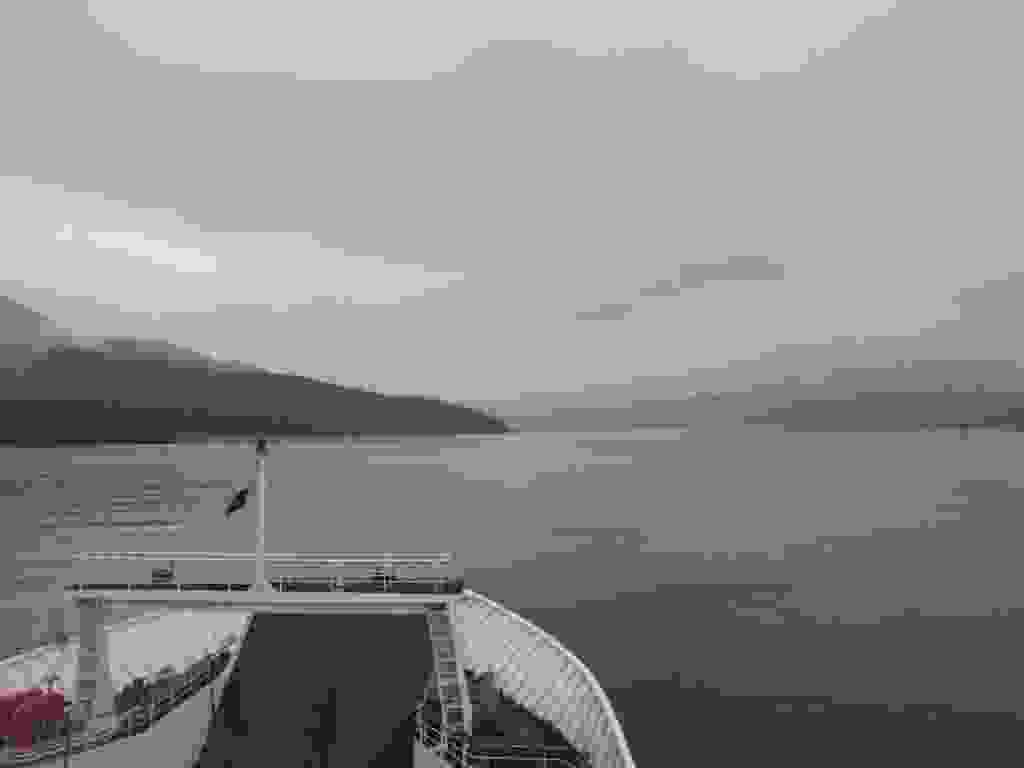
\includegraphics[width=\mywidth]{../wp-content/uploads/2015/02/P2192198.jpg} \end{center}
\vspace{-\topsep}

\pagebreak
~\\
\begin{center} 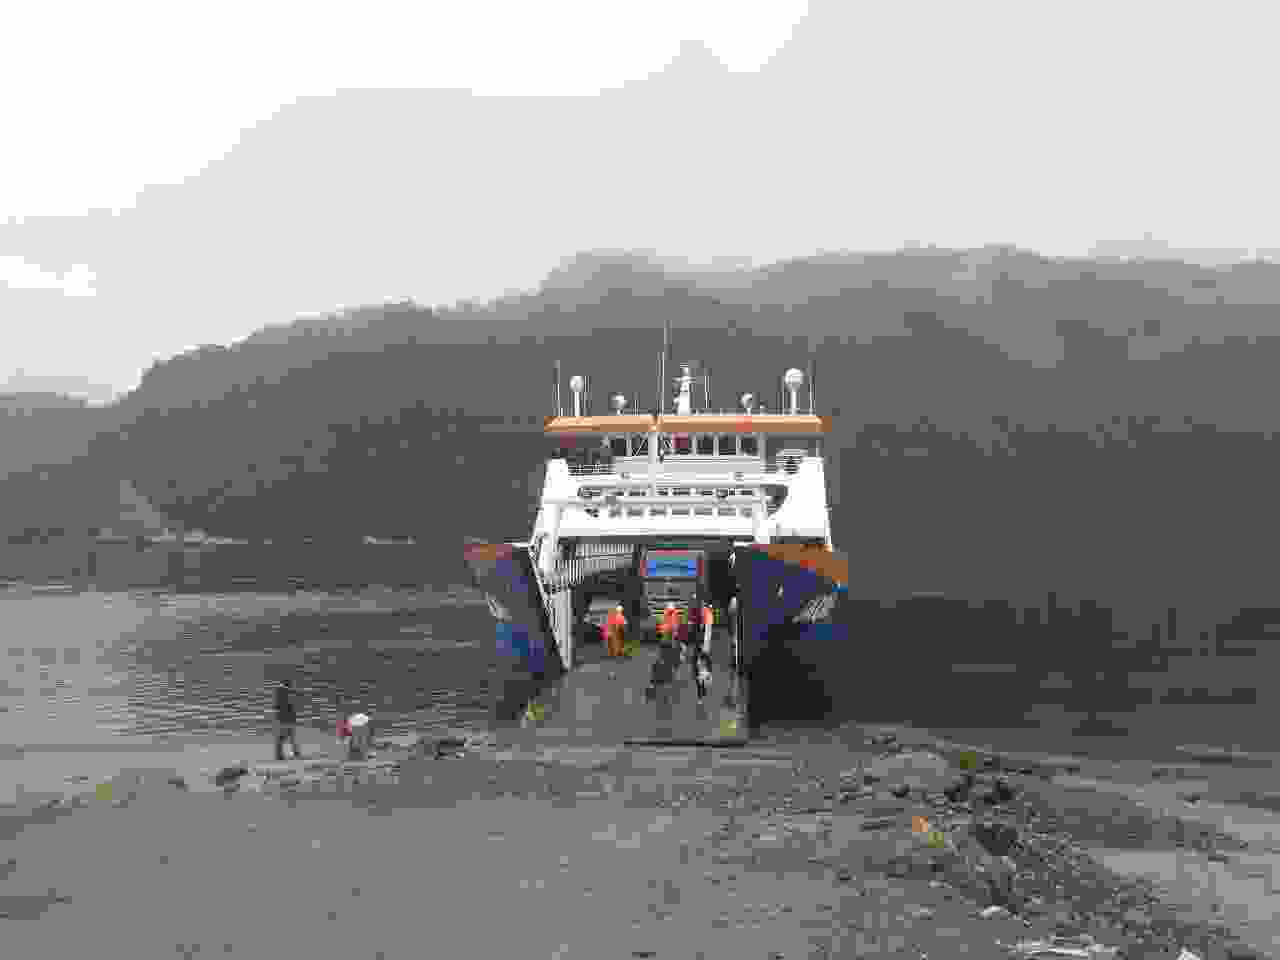
\includegraphics[width=\mywidth]{../wp-content/uploads/2015/02/P2192200.jpg} \end{center}
\begin{center} 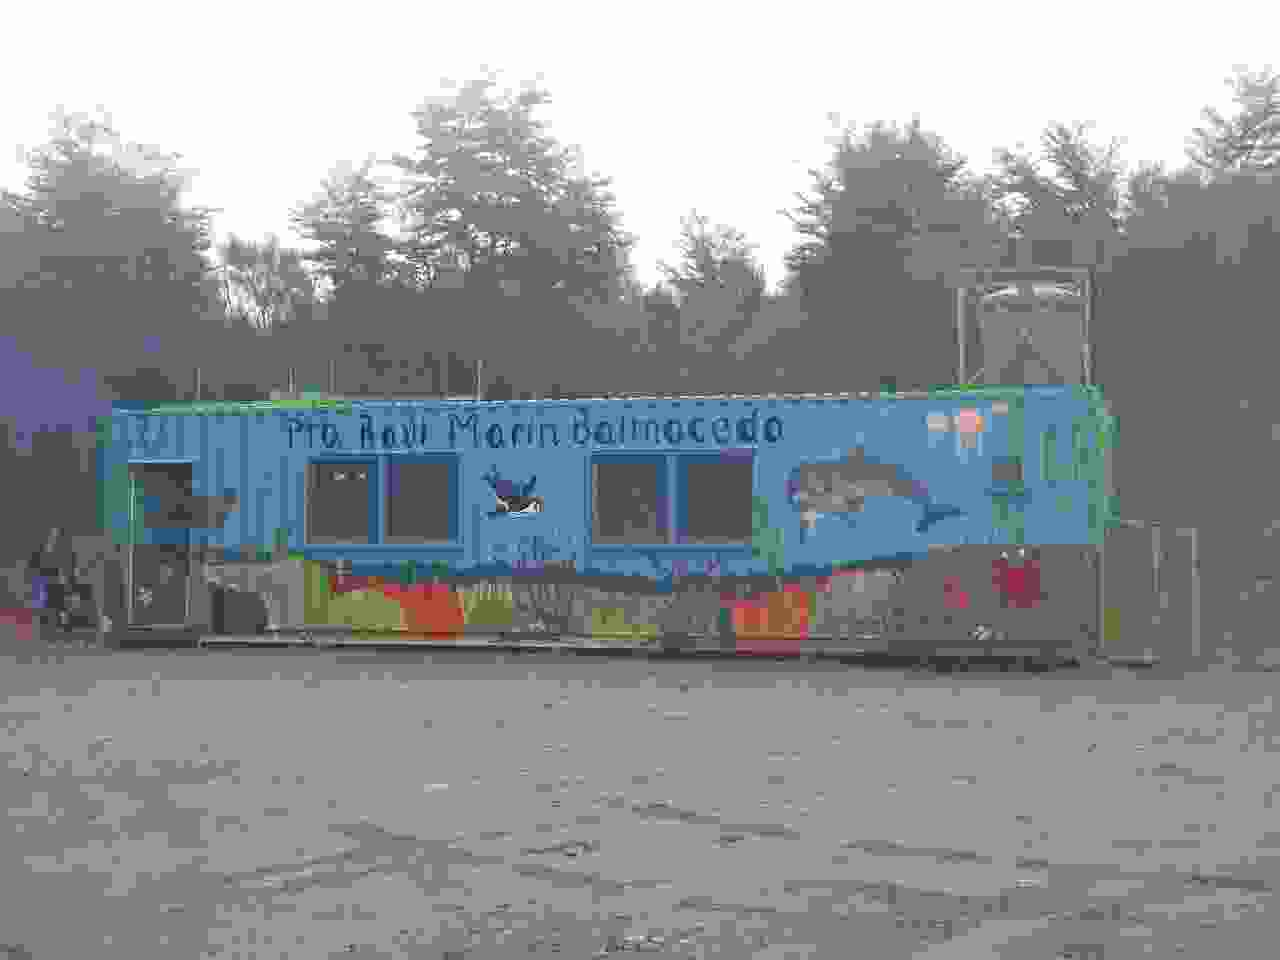
\includegraphics[width=\mywidth]{../wp-content/uploads/2015/02/P2192201.jpg} \end{center}
\vspace{-\topsep}
\vspace{-3mm}

\pagebreak
70km de piste pour rejoindre la Carretera Austral, le long de la belle rivière Palena.
\begin{center} 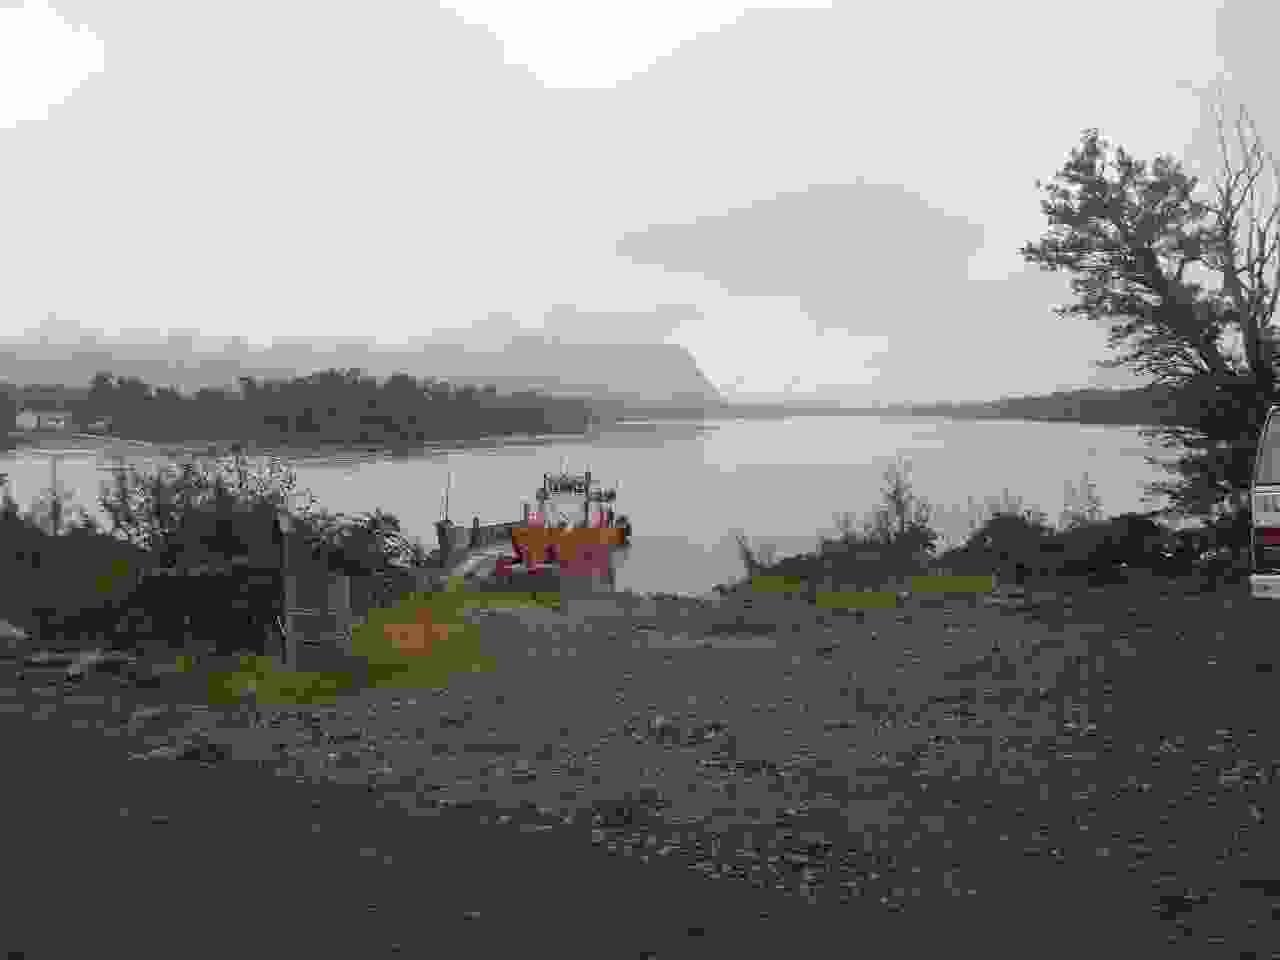
\includegraphics[width=\mywidth]{../wp-content/uploads/2015/02/P2192214.jpg} \end{center}
\begin{center} 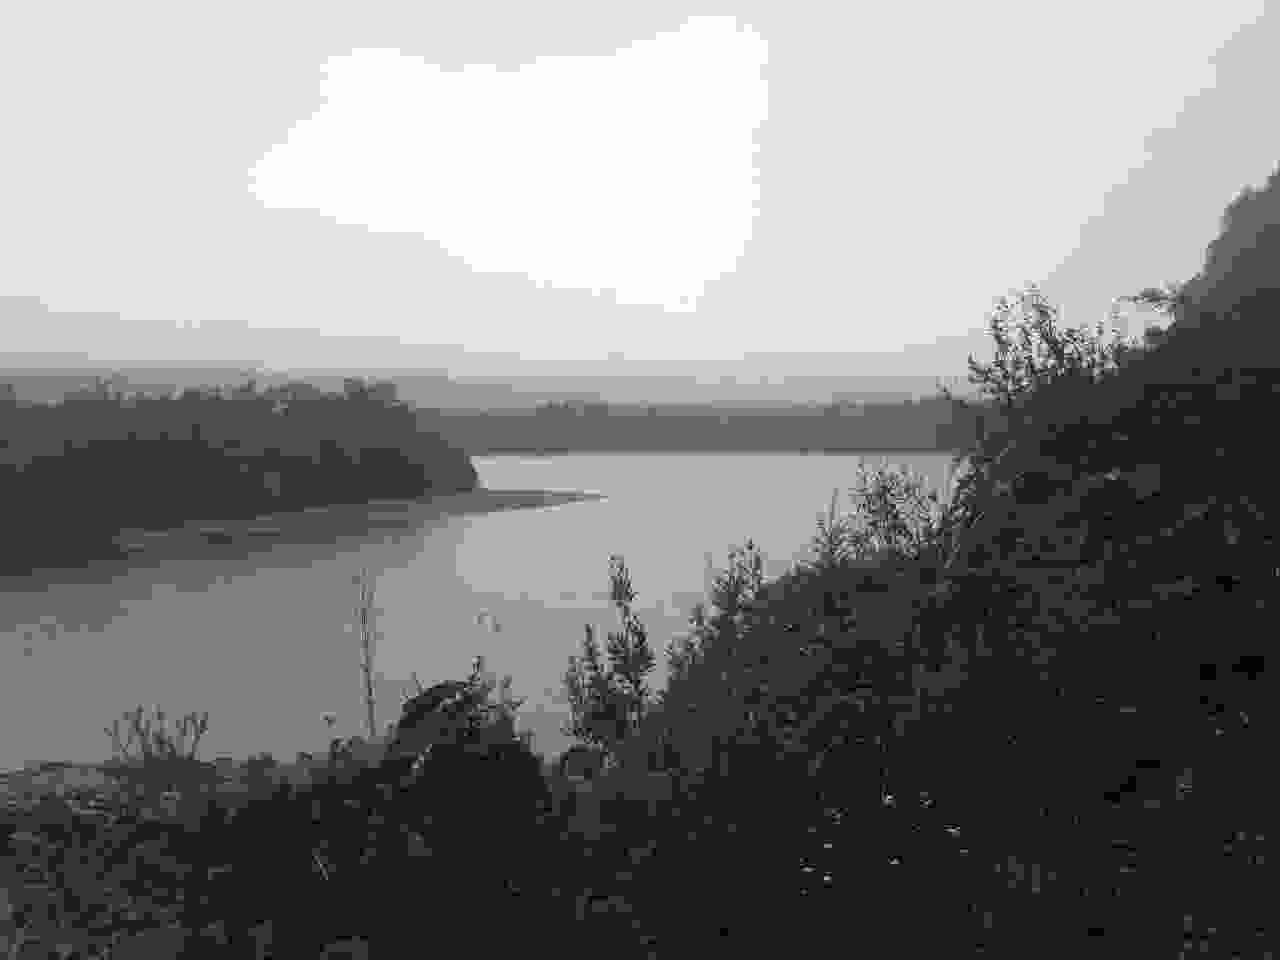
\includegraphics[width=\mywidth]{../wp-content/uploads/2015/02/P2192216.jpg} \end{center}
\vspace{-\topsep}
\vspace{-3mm}

\pagebreak
~
\begin{center} 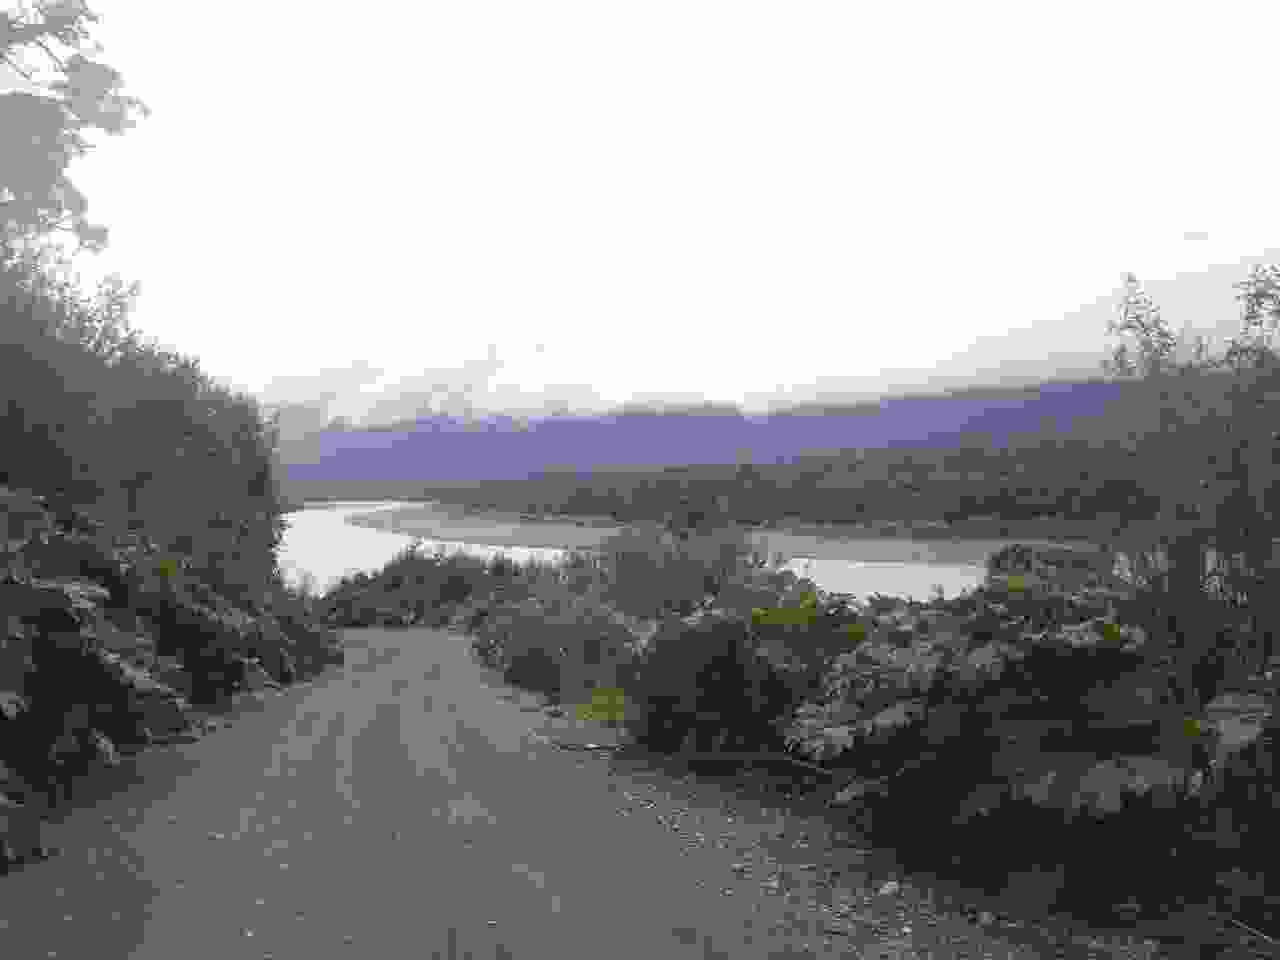
\includegraphics[width=\mywidth]{../wp-content/uploads/2015/02/P2192220.jpg} \end{center}
\begin{center} 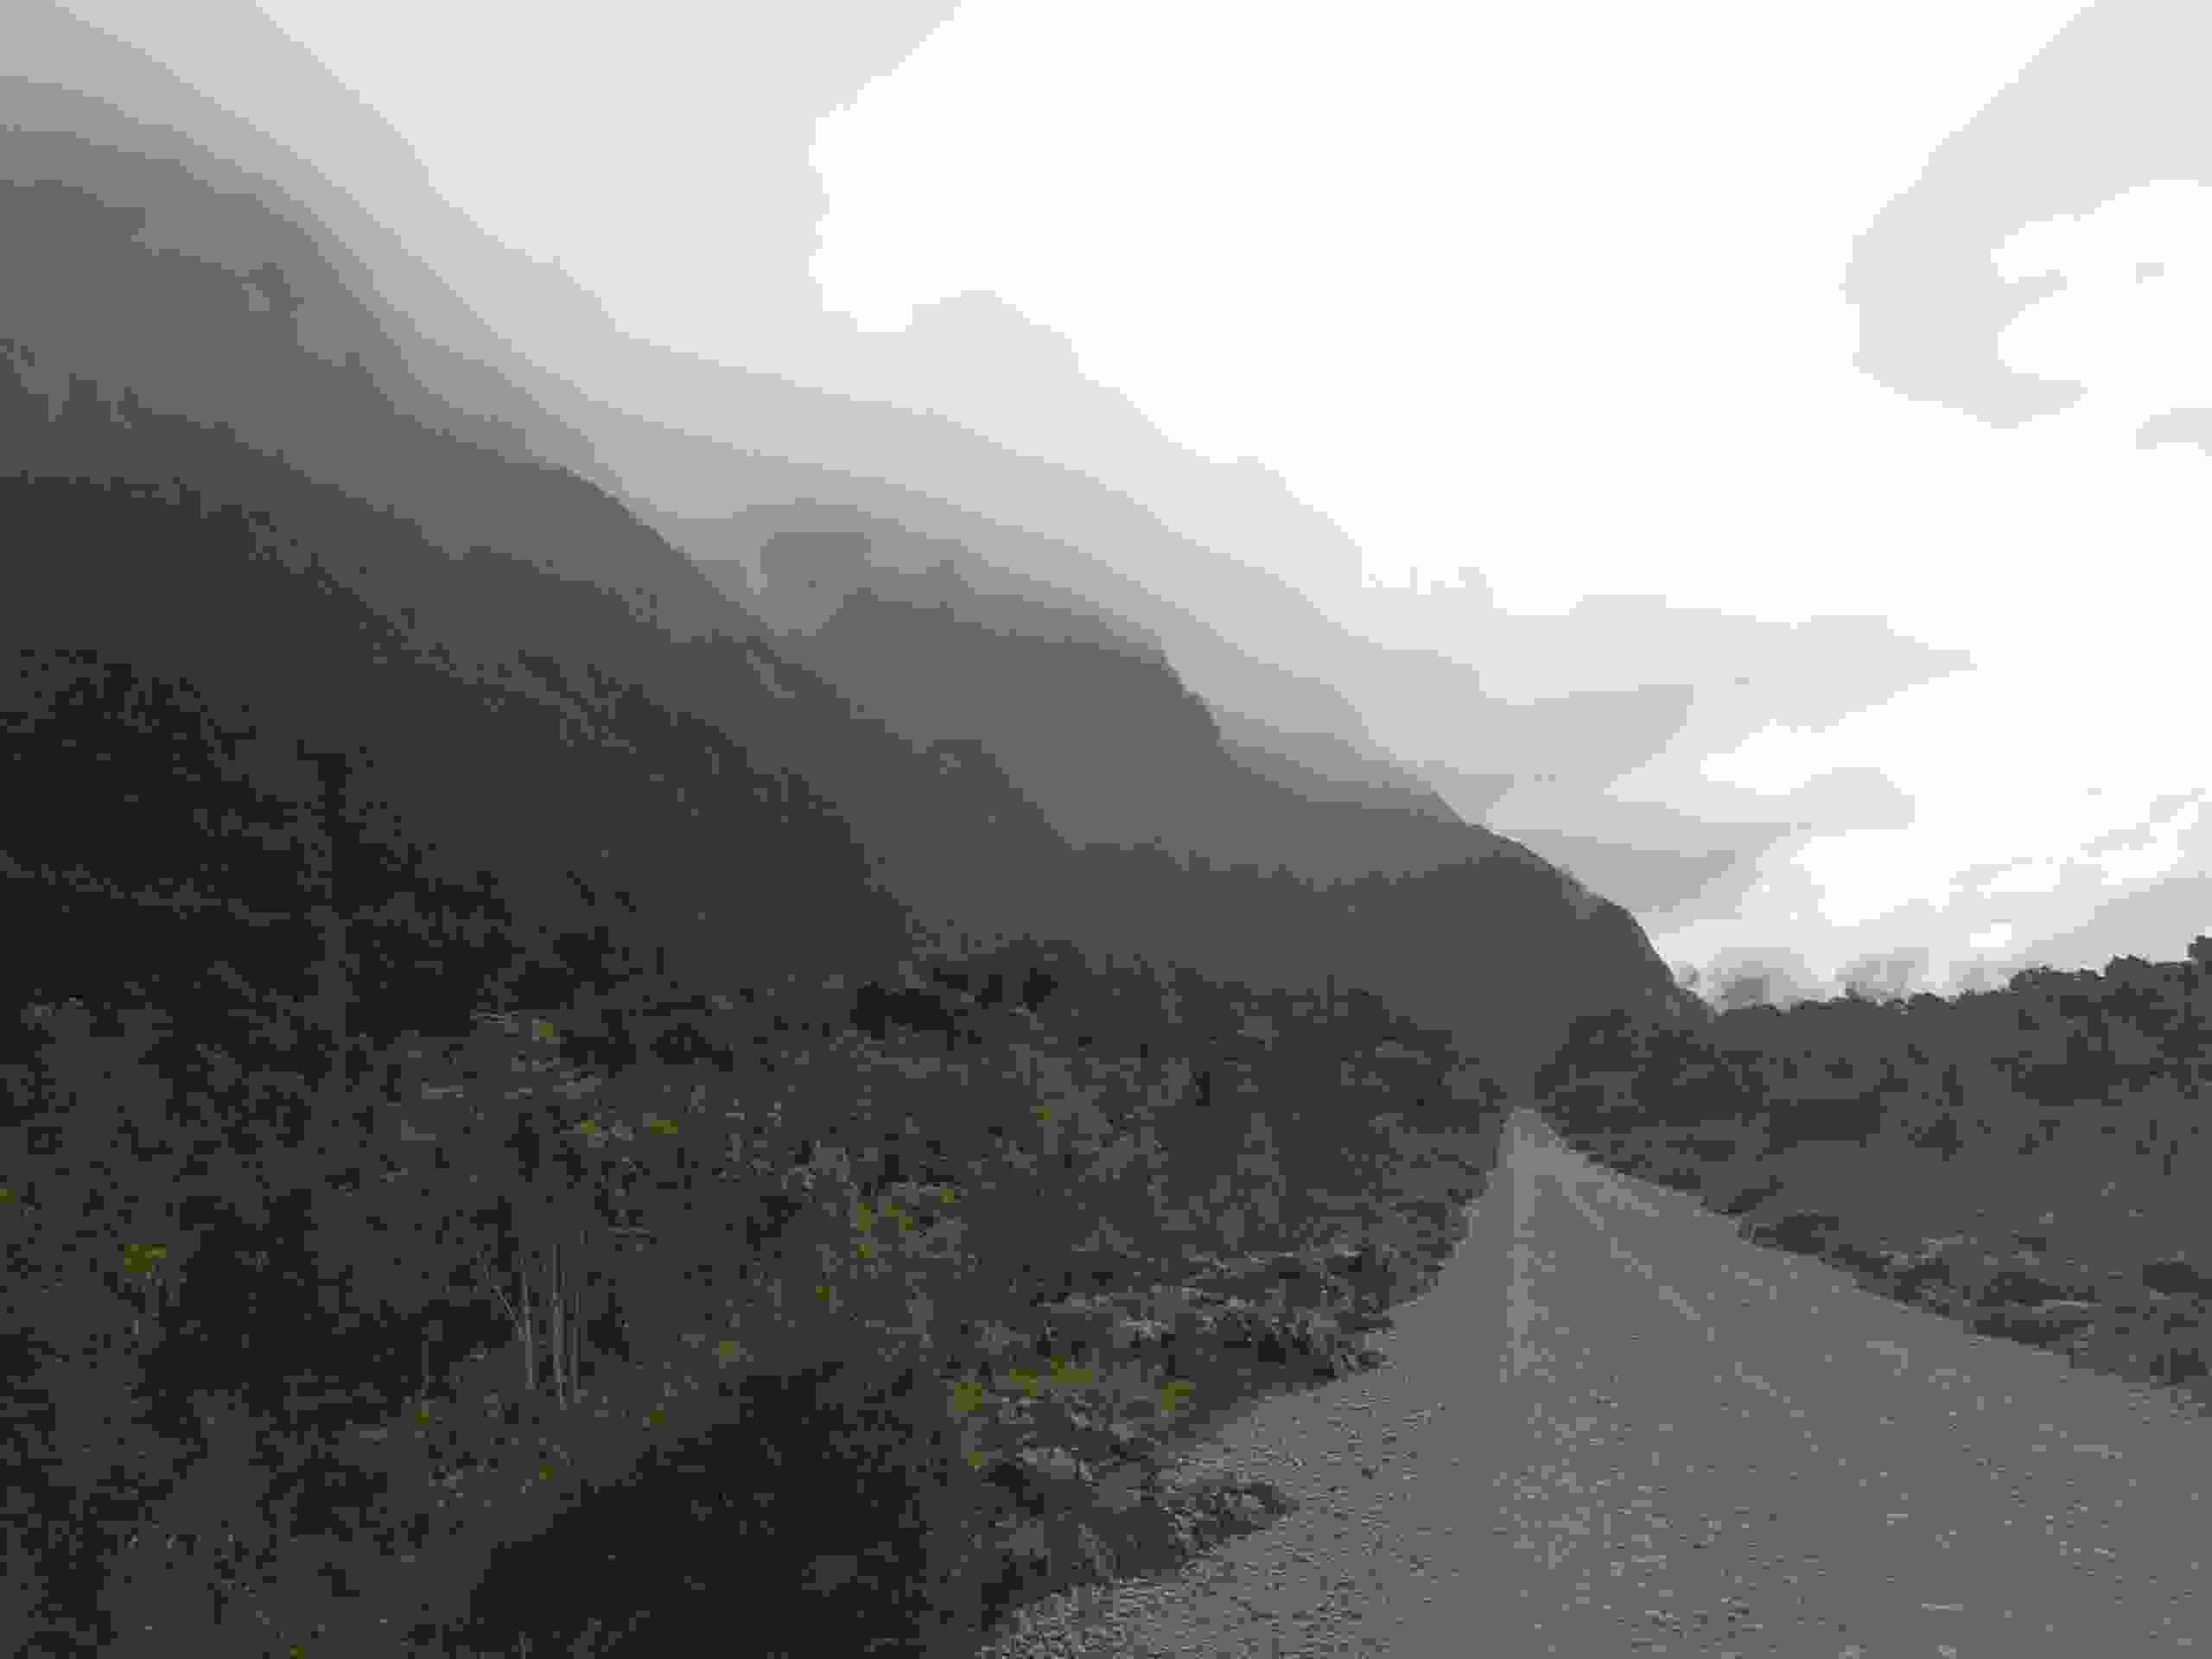
\includegraphics[width=\mywidth]{../wp-content/uploads/2015/02/P2192227.jpg} \end{center}
\vspace{-\topsep}
\vspace{-3.5mm}

\pagebreak
 Superbe bivouac au bord de l'eau.
\begin{center} 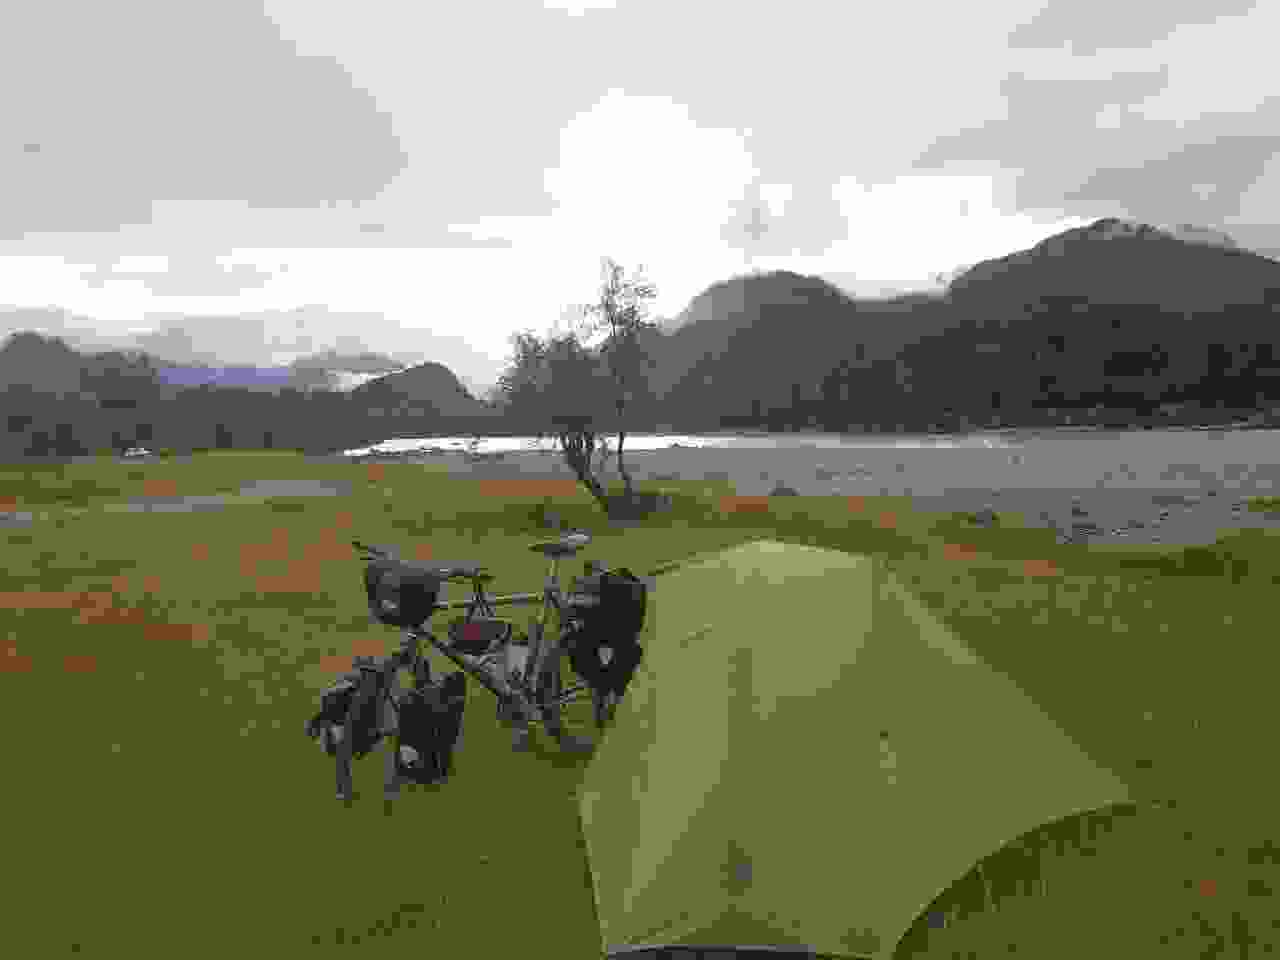
\includegraphics[width=\mywidth]{../wp-content/uploads/2015/02/P2202230.jpg} \end{center}
\begin{center} 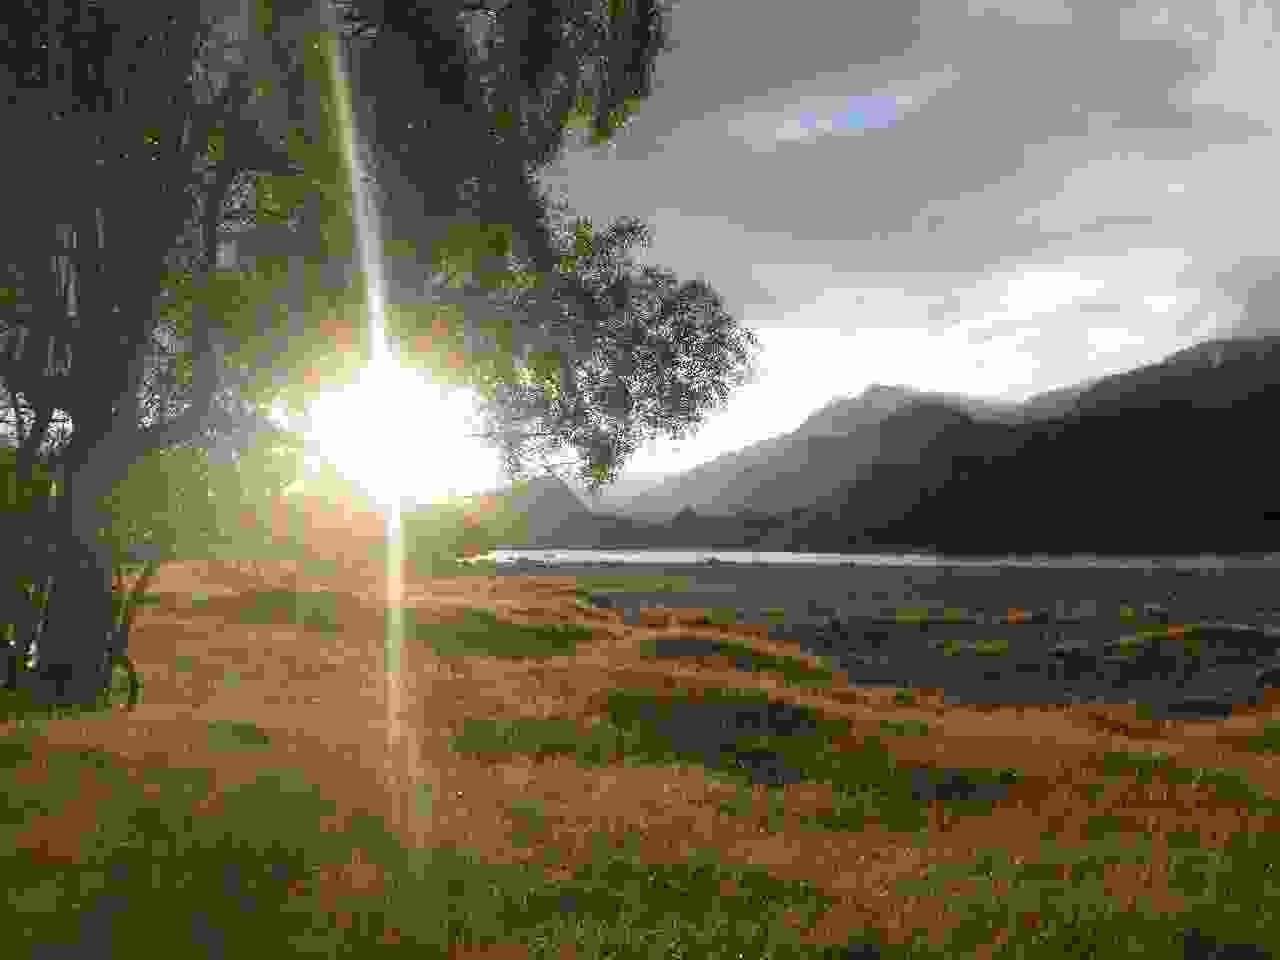
\includegraphics[width=\mywidth]{../wp-content/uploads/2015/02/P2202236.jpg} \end{center}
\begin{center} 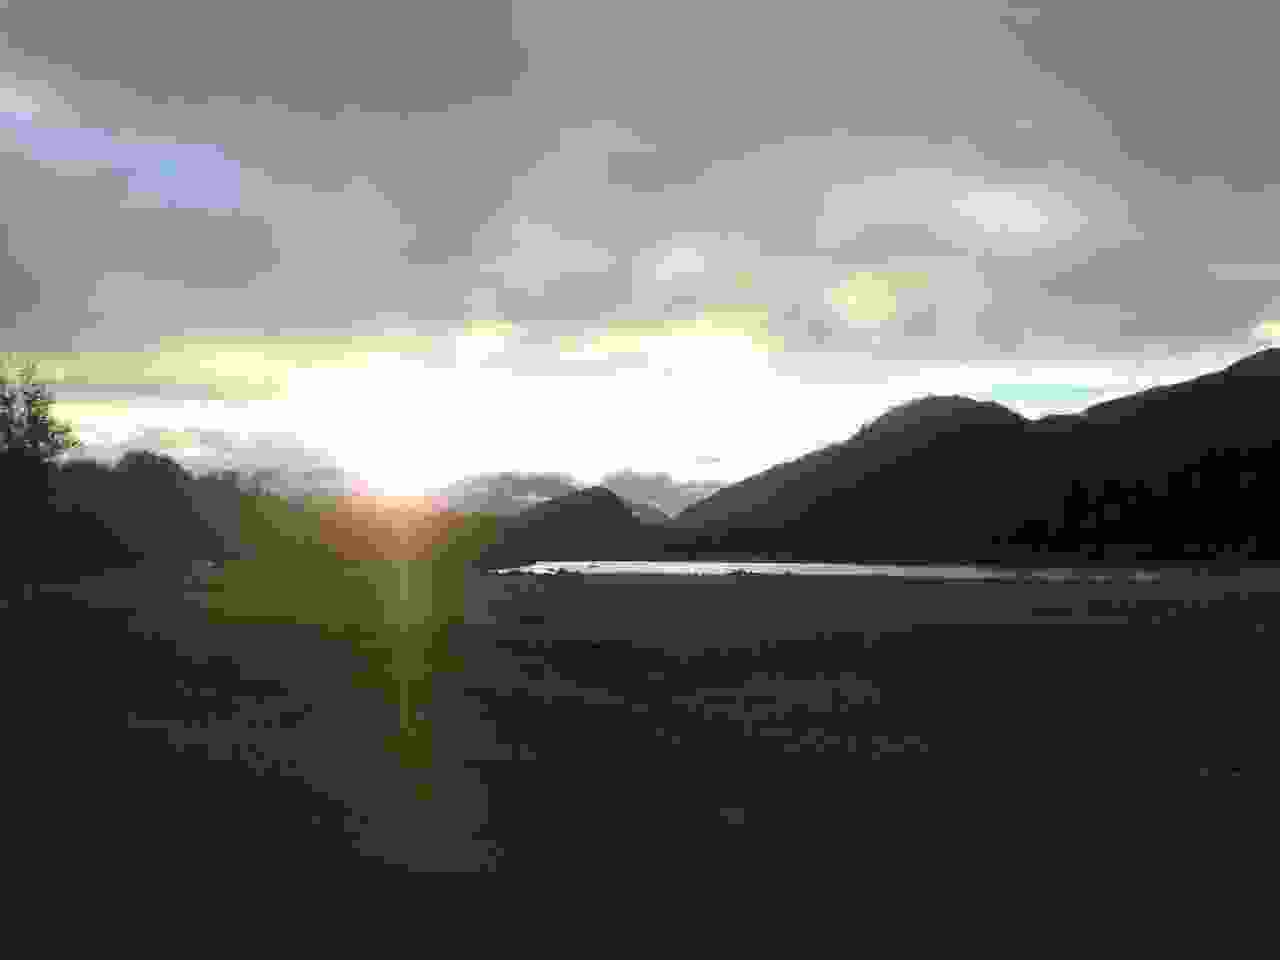
\includegraphics[width=\mywidth]{../wp-content/uploads/2015/02/P2202242.jpg} \end{center}
\begin{center} 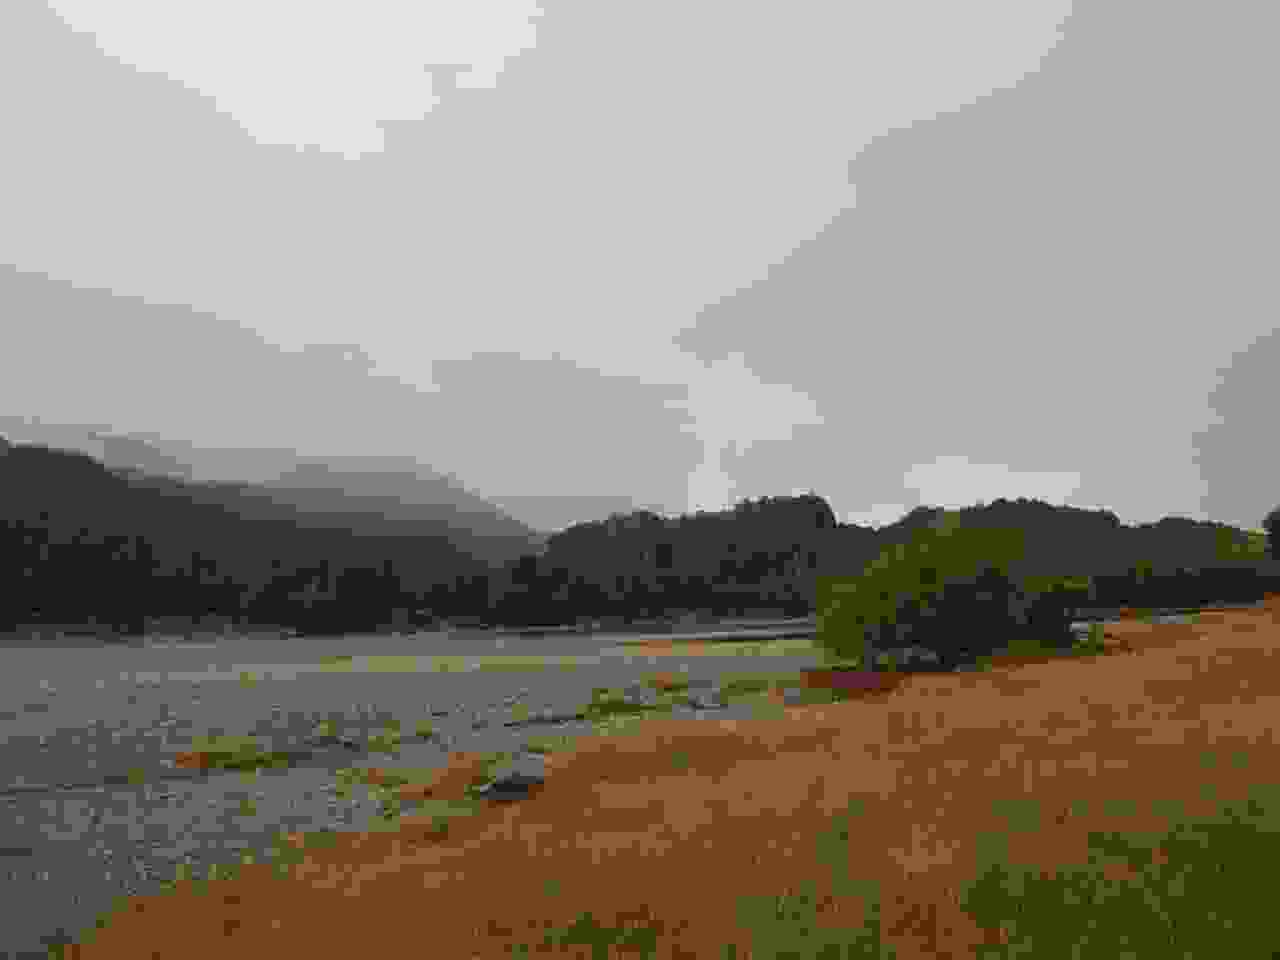
\includegraphics[width=\mywidth]{../wp-content/uploads/2015/02/P22022451.jpg} \end{center}
\begin{center} 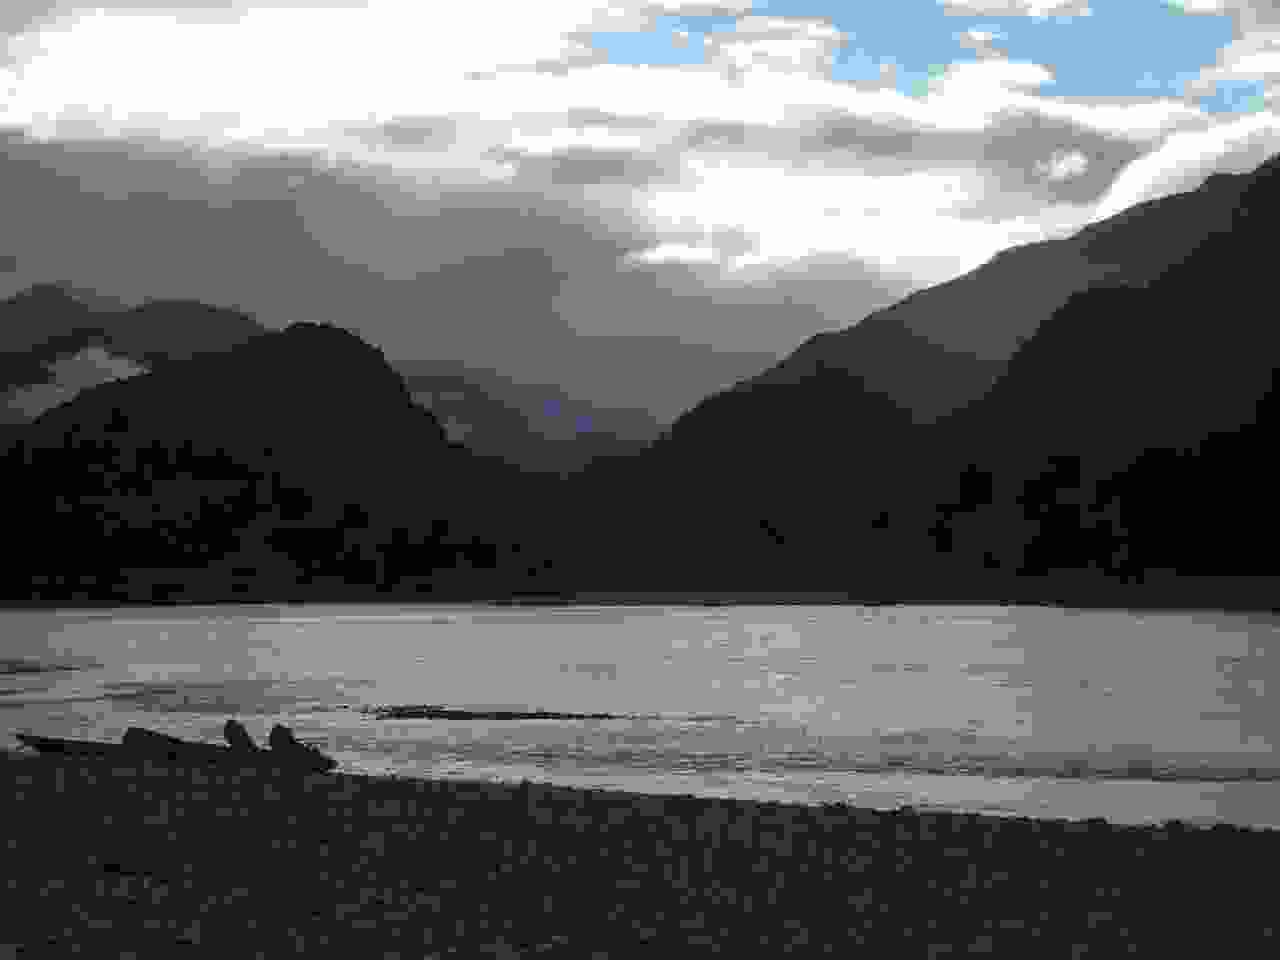
\includegraphics[width=\mywidth]{../wp-content/uploads/2015/02/P2202234.jpg} \end{center}

Première étape sur la Carretera entre La Junta et Villa Santa Lucia.
\begin{center} 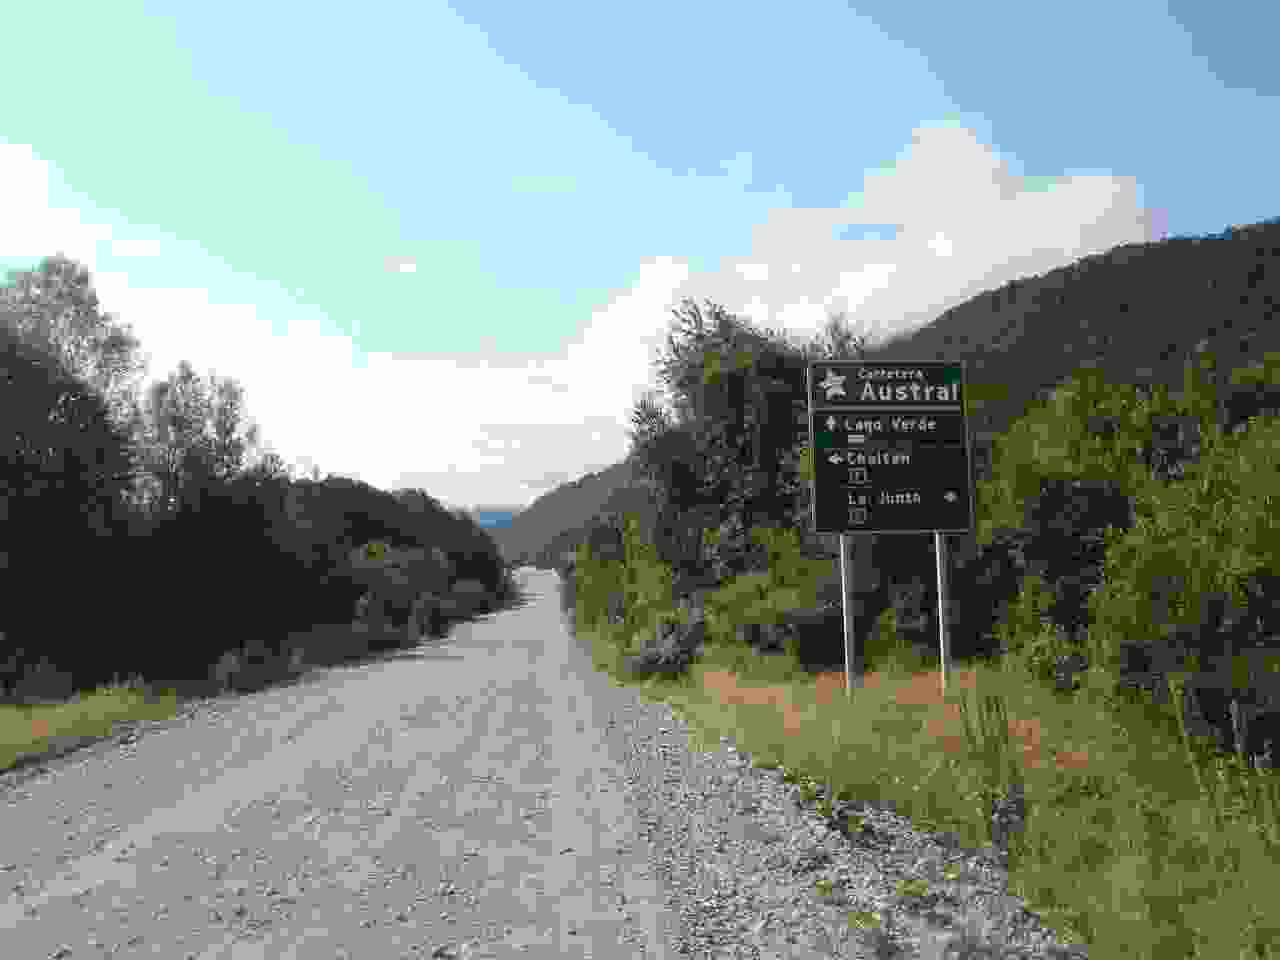
\includegraphics[width=\mywidth]{../wp-content/uploads/2015/02/P2202251.jpg} \end{center}
\begin{center} 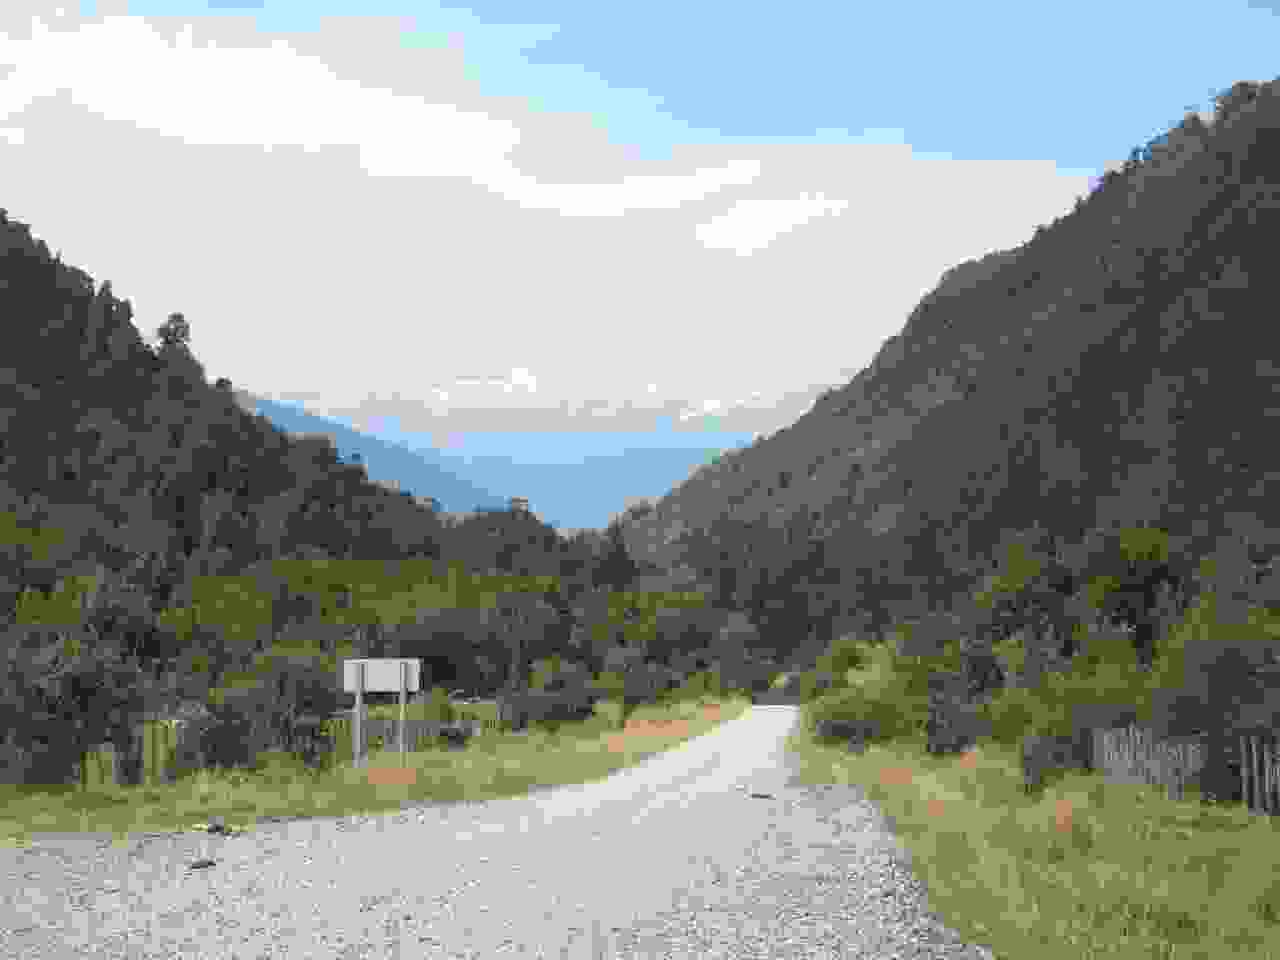
\includegraphics[width=\mywidth]{../wp-content/uploads/2015/02/P2202258.jpg} \end{center}
\begin{center} 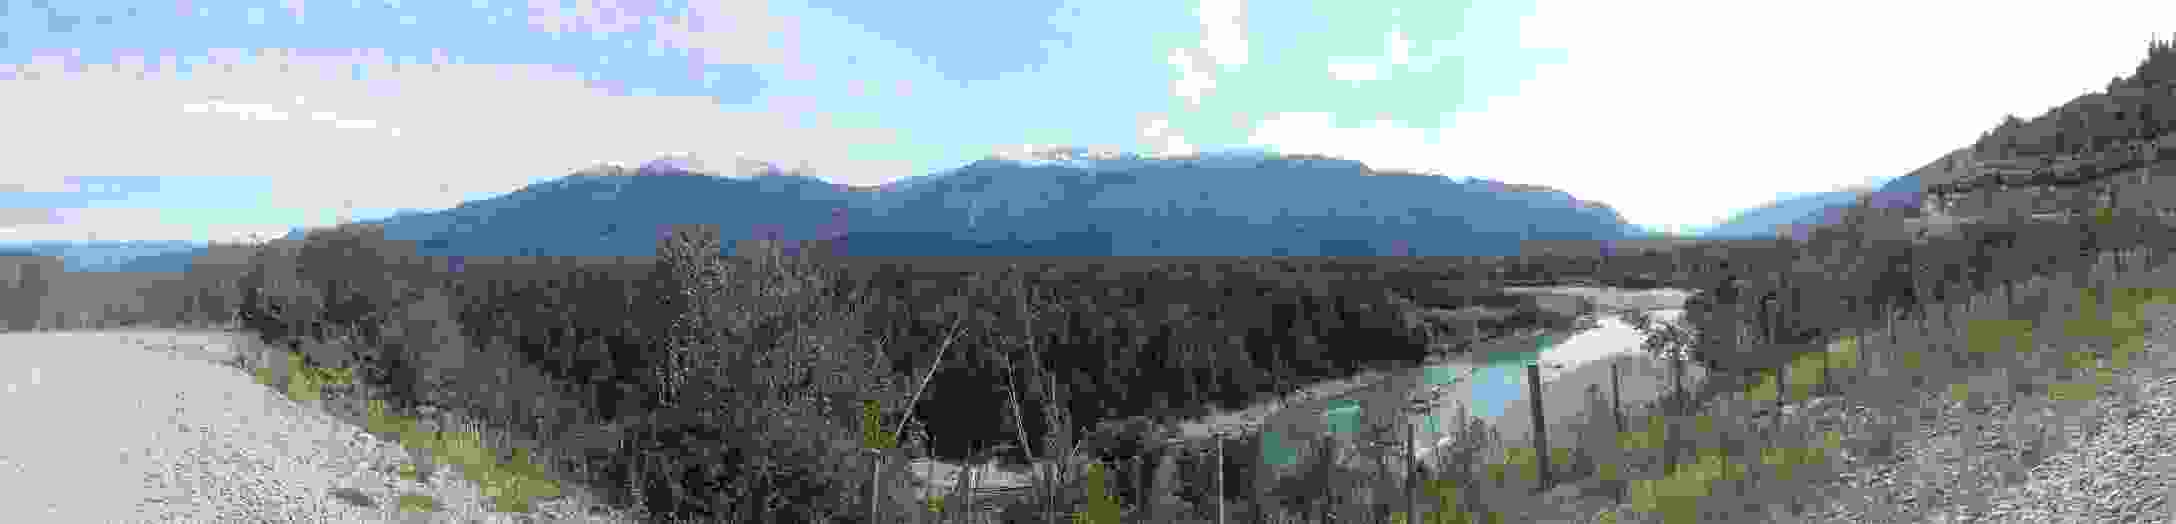
\includegraphics[width=\textwidth]{../wp-content/uploads/2015/02/P2202254.jpg} \end{center}
\begin{center} 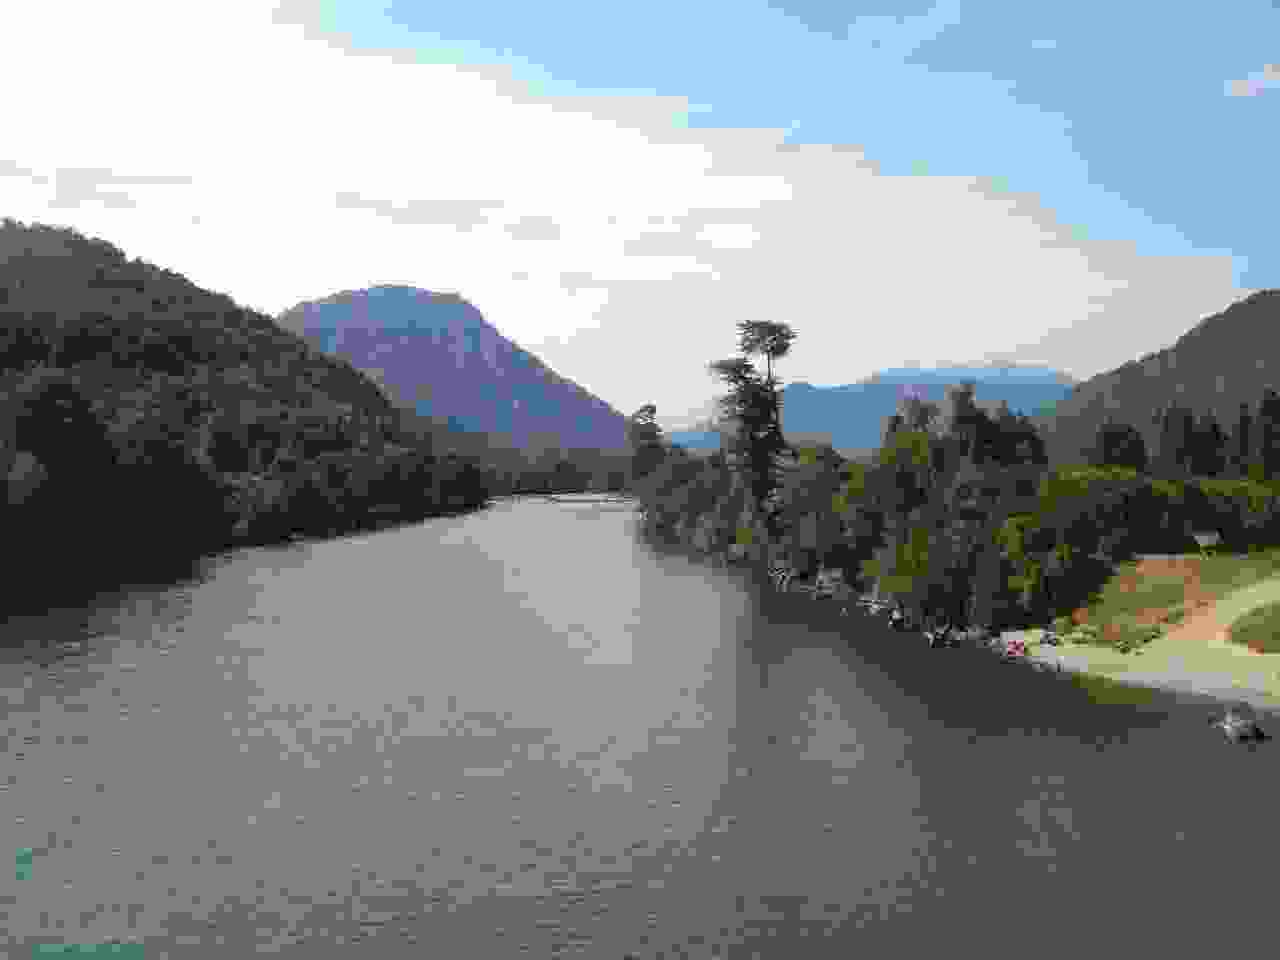
\includegraphics[width=\mywidth]{../wp-content/uploads/2015/02/P2202253.jpg} \end{center}
\begin{center} 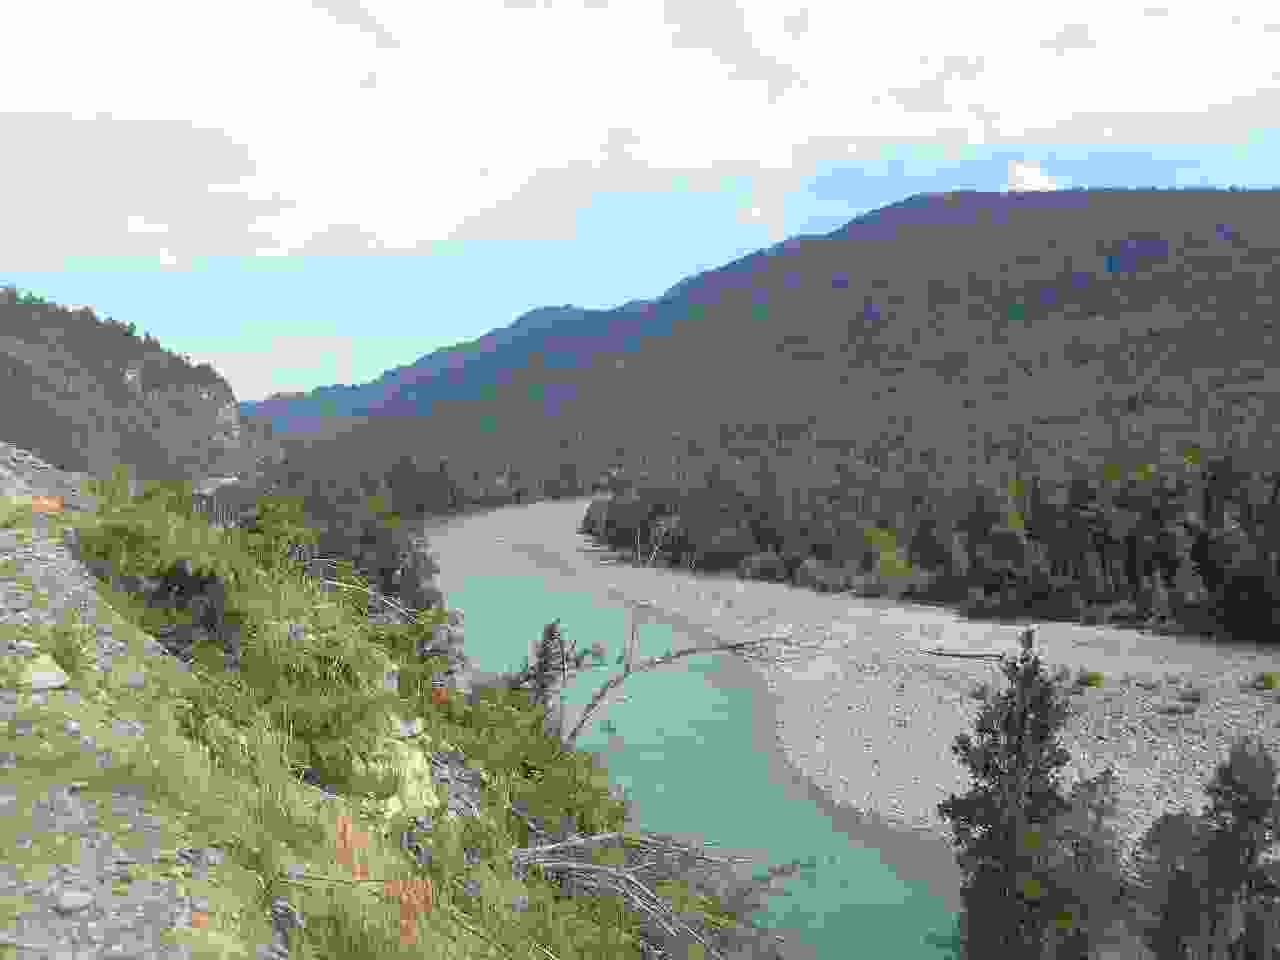
\includegraphics[width=\mywidth]{../wp-content/uploads/2015/02/P2202260.jpg} \end{center}
\begin{center} 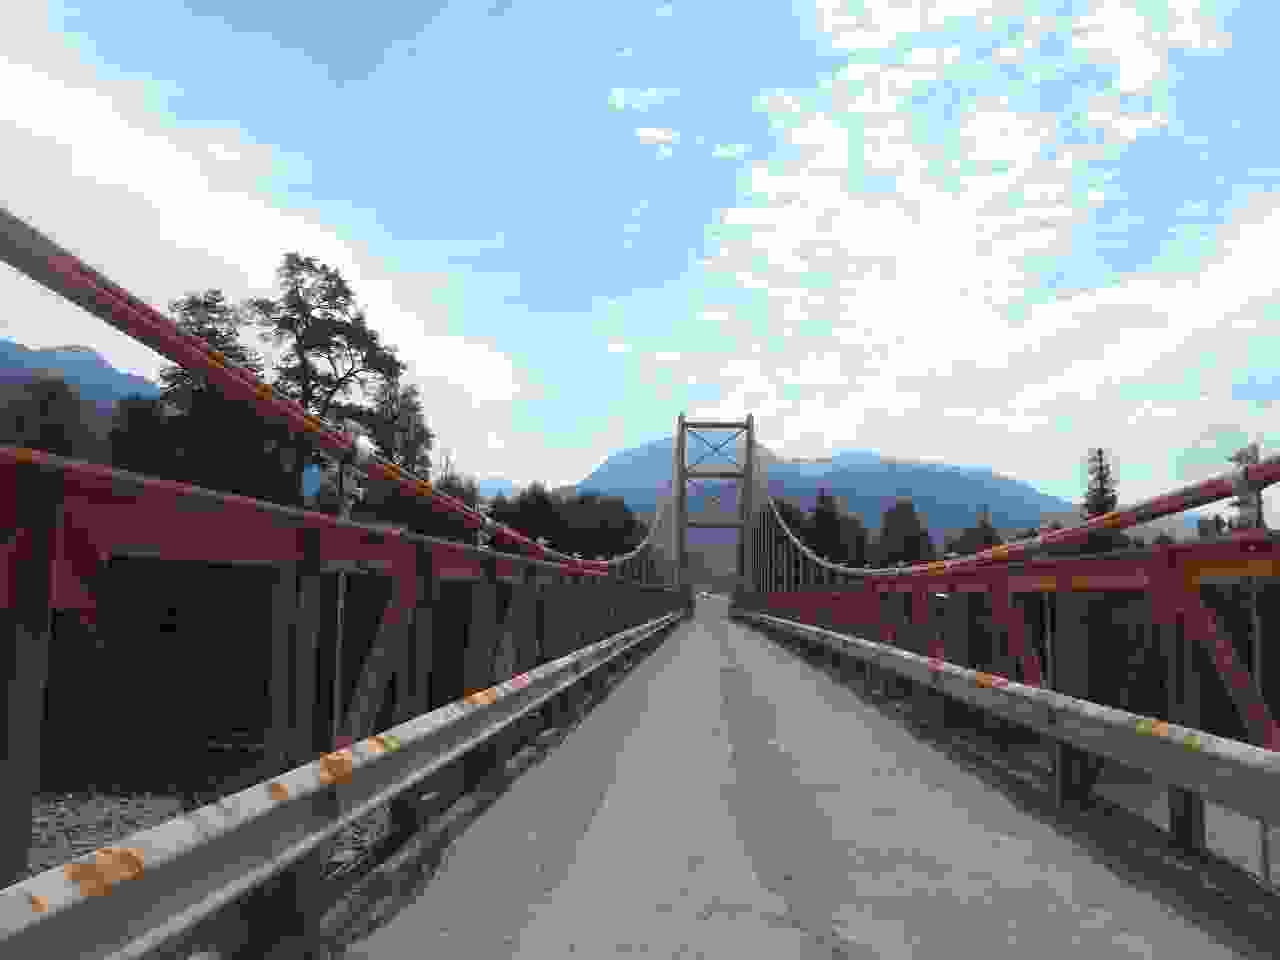
\includegraphics[width=\mywidth]{../wp-content/uploads/2015/02/P2202262.jpg} \end{center}
\vspace{-\topsep}
\vspace{-8.5mm}

\pagebreak
~
\begin{center} 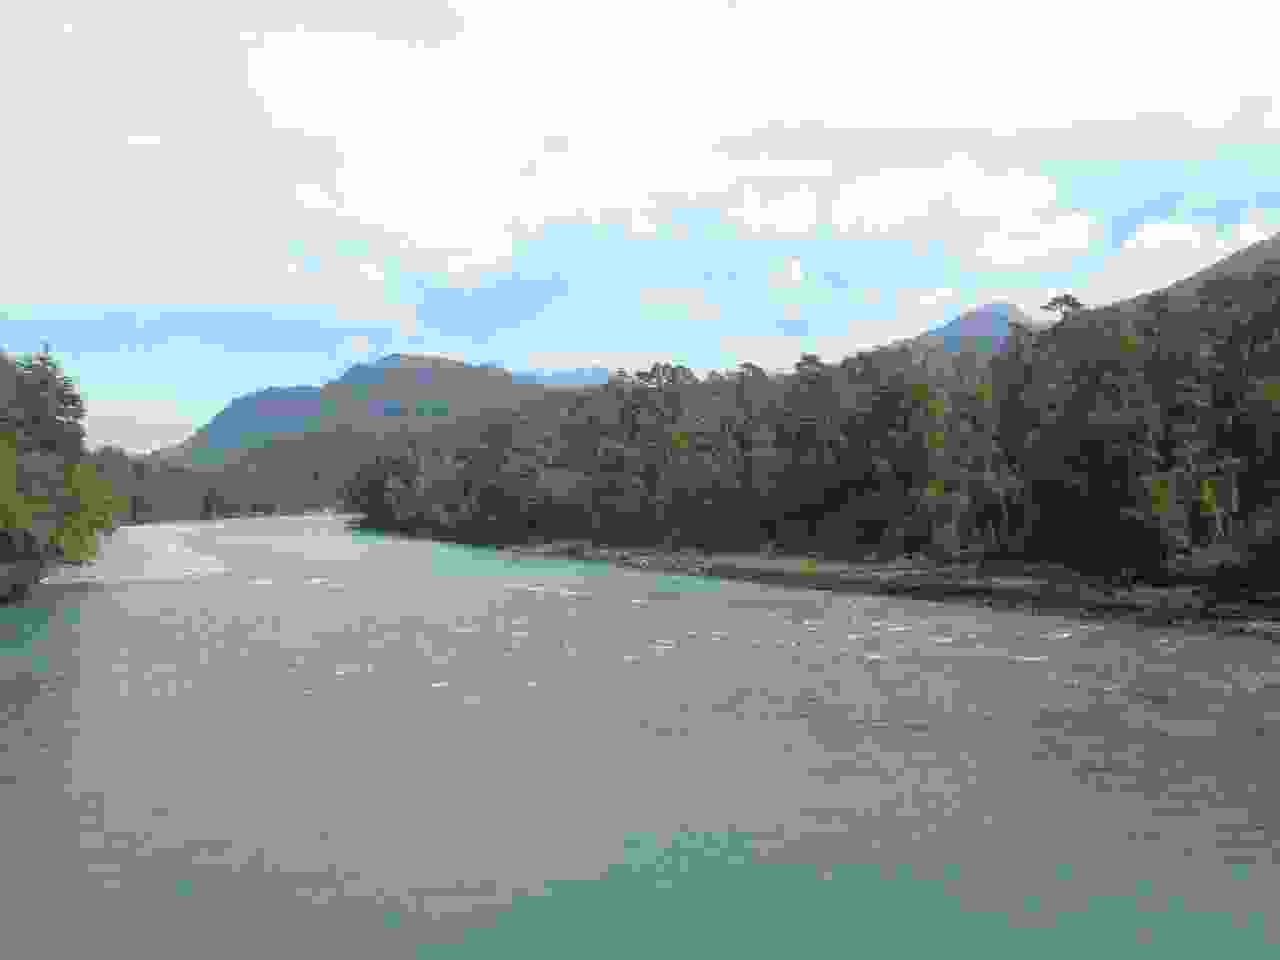
\includegraphics[width=\mywidth]{../wp-content/uploads/2015/02/P2202263.jpg} \end{center}
\begin{center} 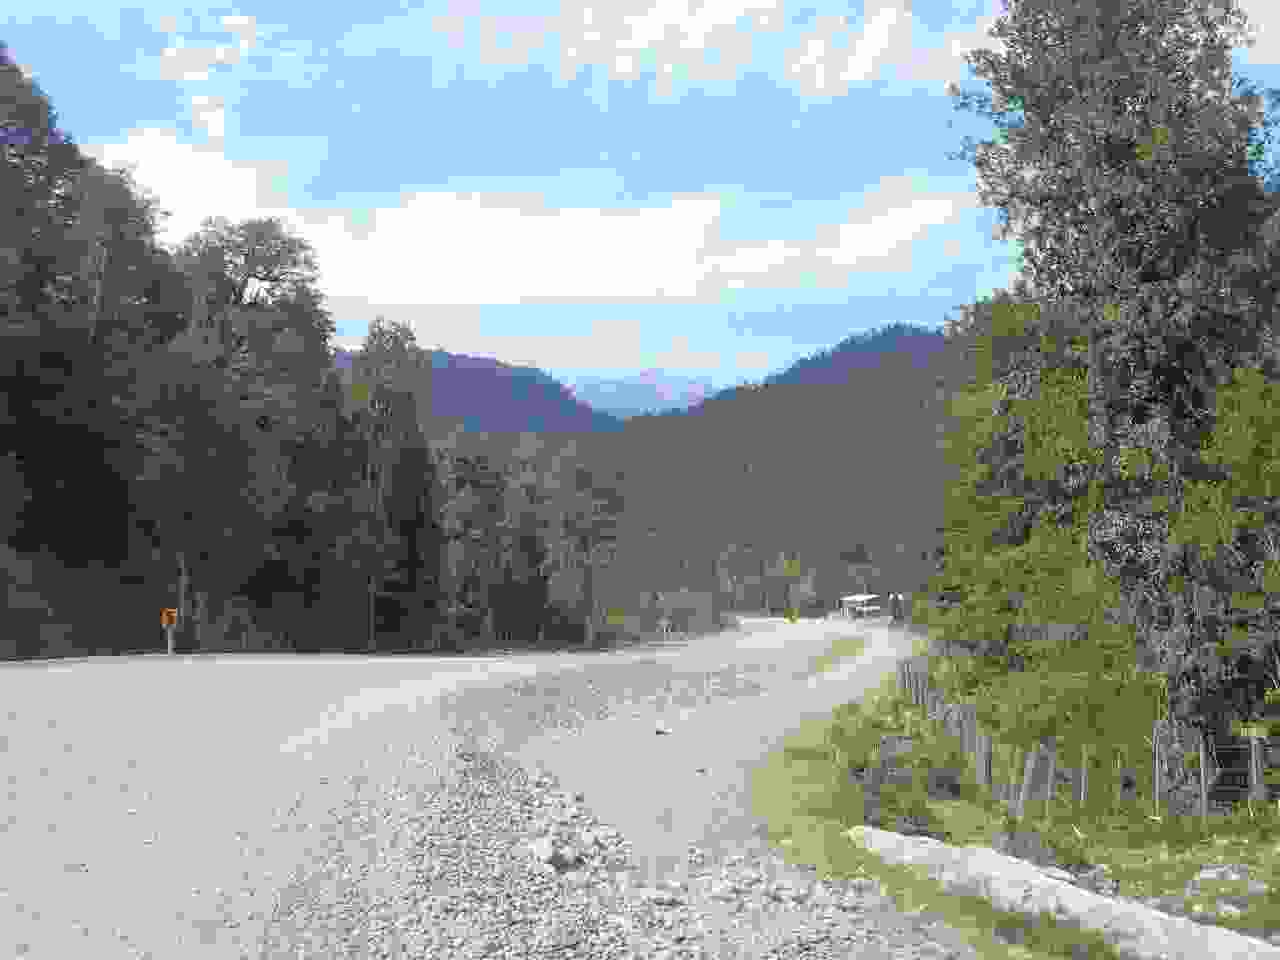
\includegraphics[width=\mywidth]{../wp-content/uploads/2015/02/P2202264.jpg} \end{center}
\vspace{-\topsep}
\vspace{-3.25mm}

\pagebreak
Le passage de la piste à la route qui fait plaisir !
\begin{center} 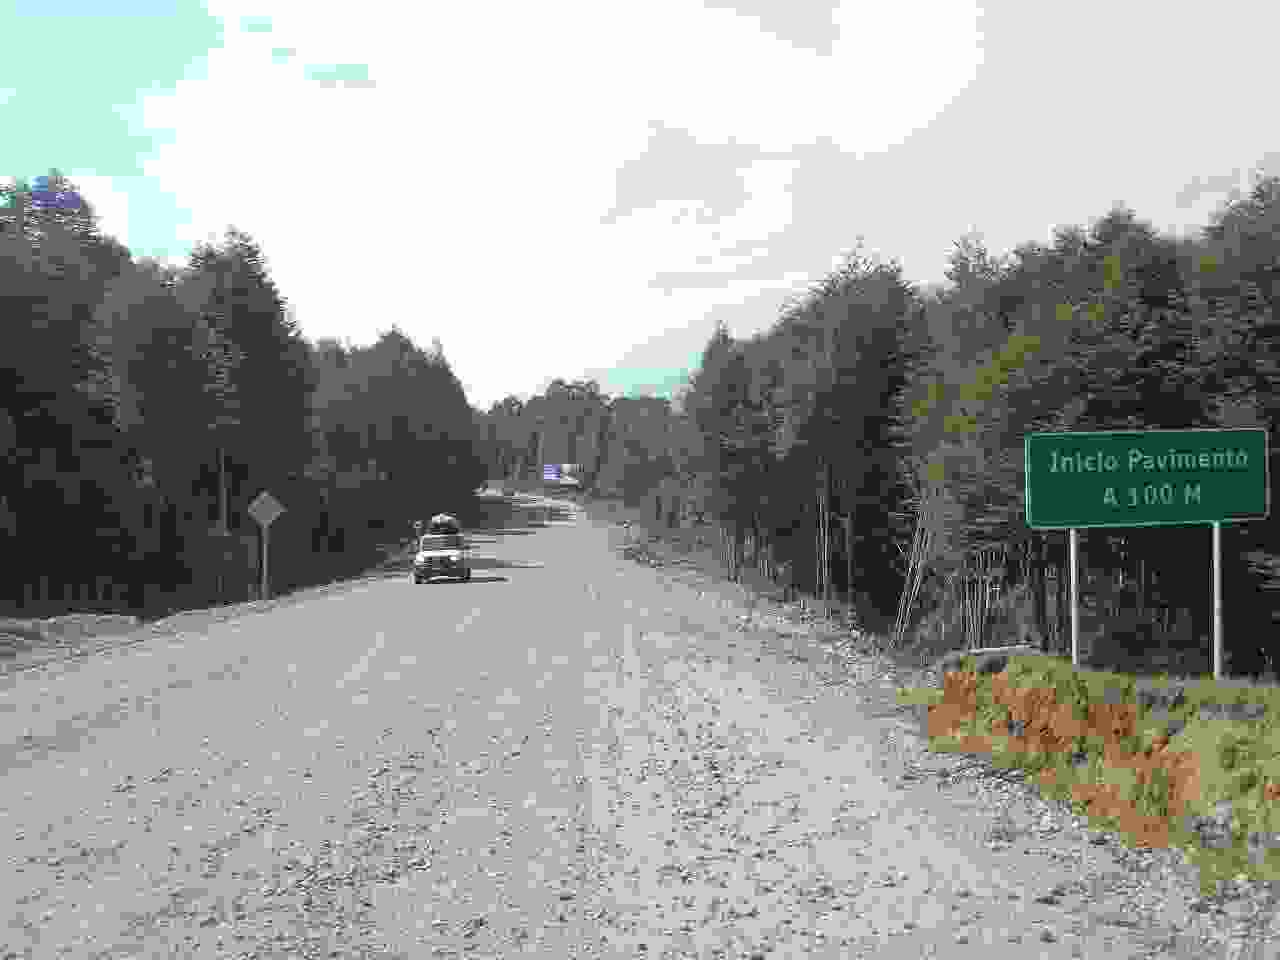
\includegraphics[width=\mywidth]{../wp-content/uploads/2015/02/P2202265.jpg} \end{center}
\begin{center} 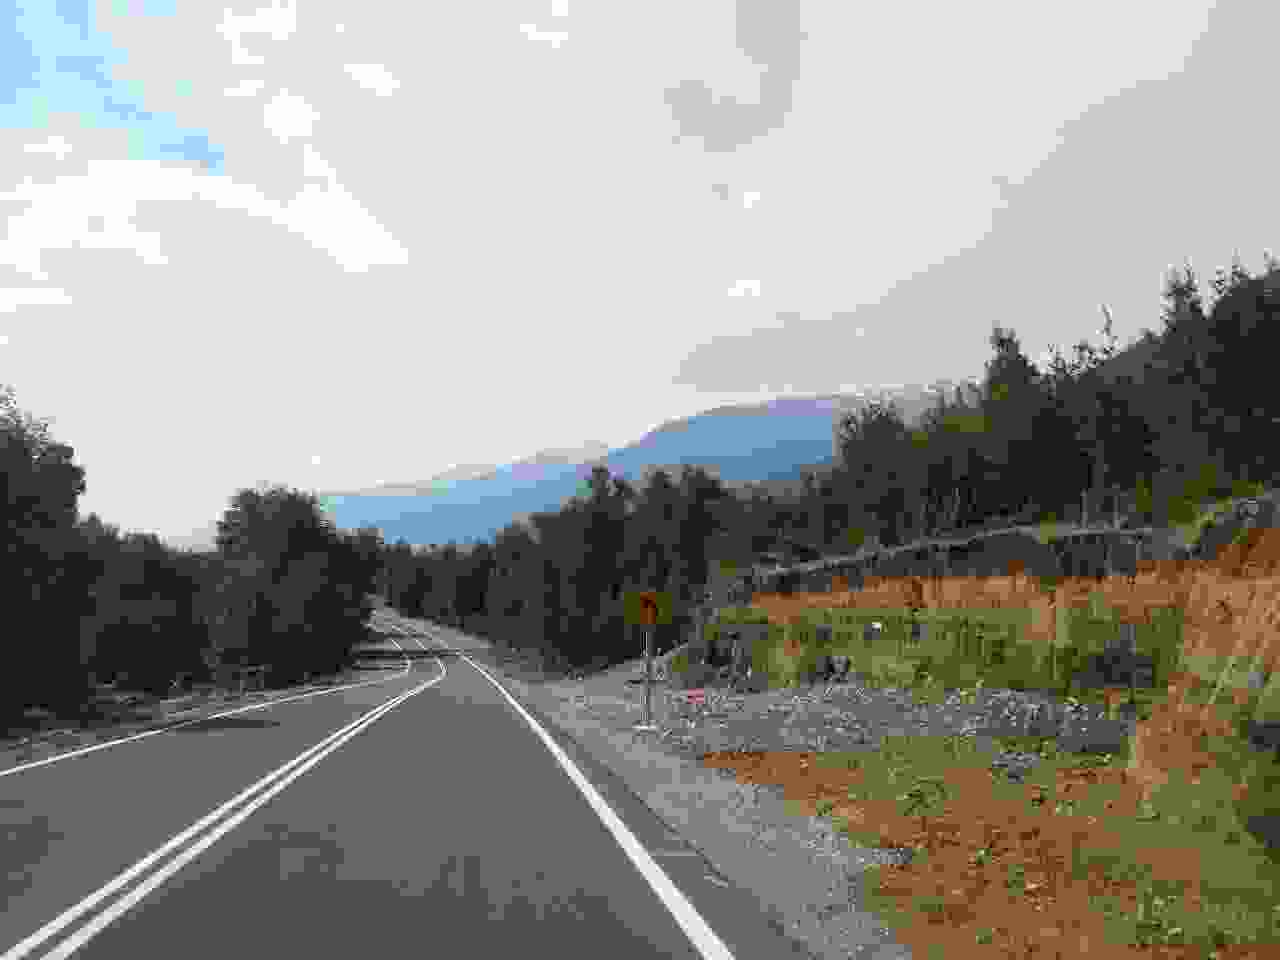
\includegraphics[width=\mywidth]{../wp-content/uploads/2015/02/P2202266.jpg} \end{center}
\vspace{-\topsep}
\vspace{-3.25mm}

\pagebreak
~
\begin{center} 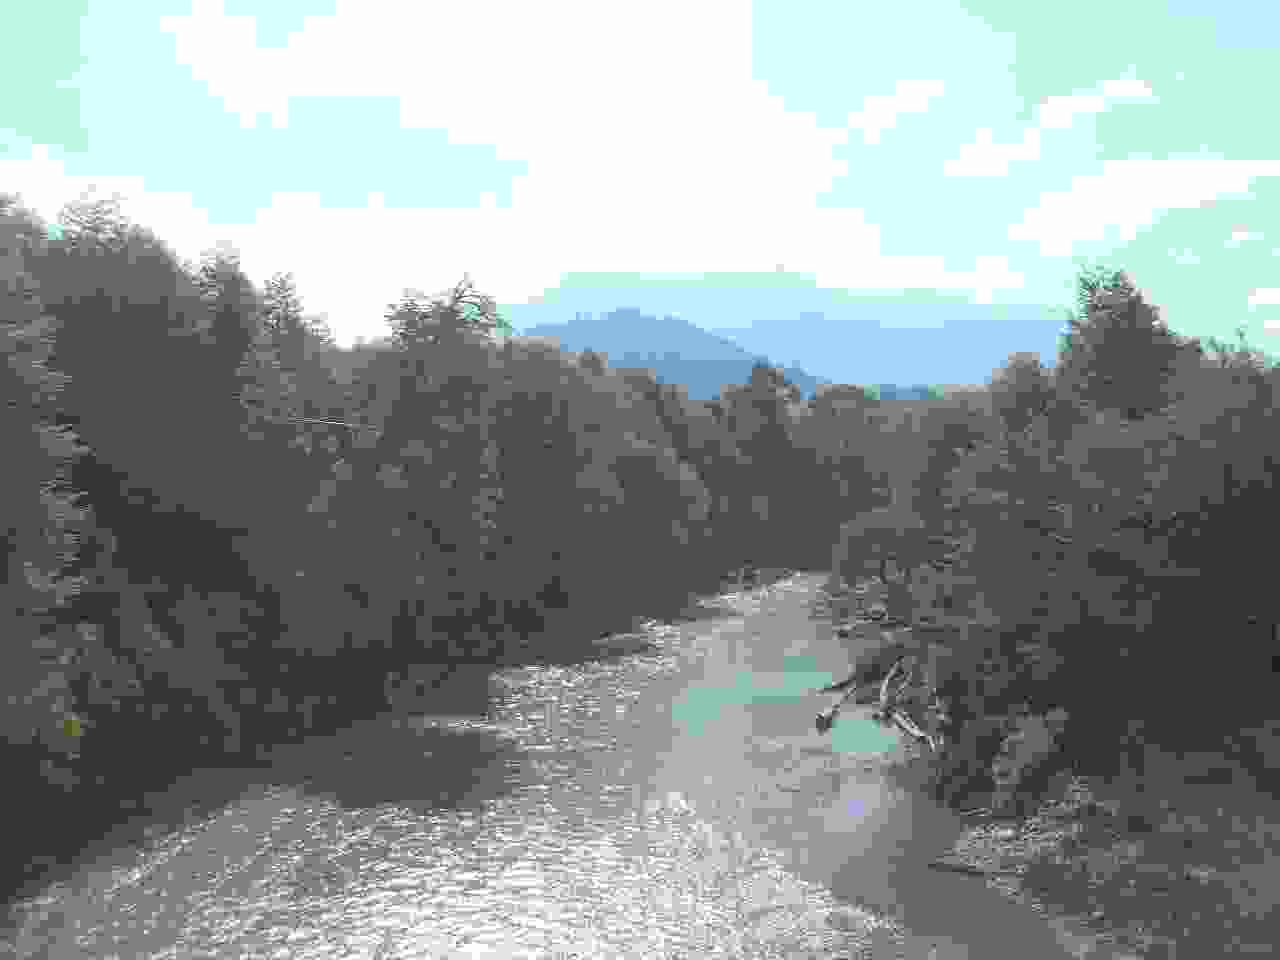
\includegraphics[width=\mywidth]{../wp-content/uploads/2015/02/P2202267.jpg} \end{center}
~
\begin{center} 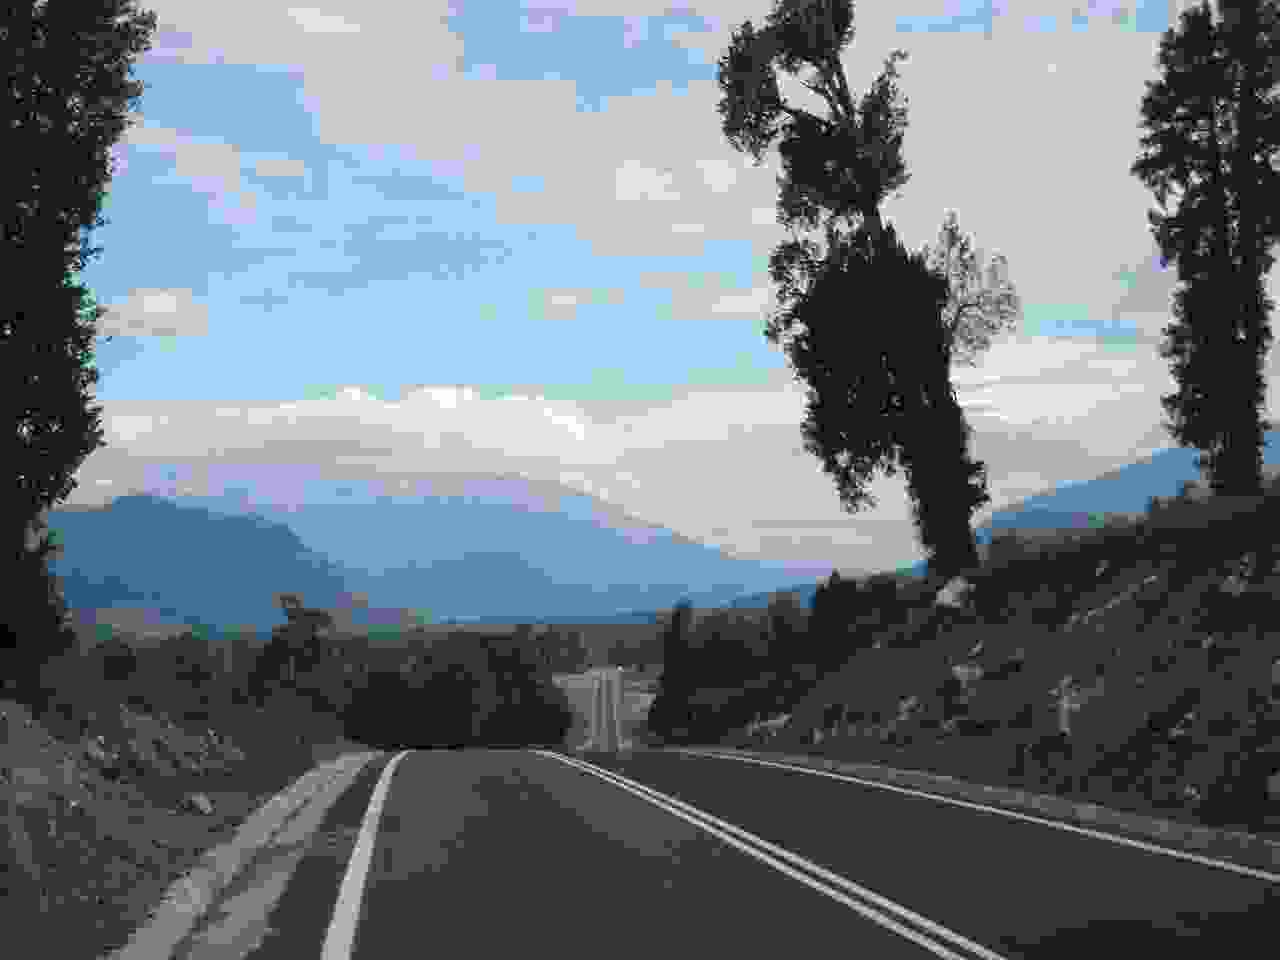
\includegraphics[width=\mywidth]{../wp-content/uploads/2015/02/P2202269.jpg} \end{center}
\vspace{-\topsep}

\pagebreak
Pas mal d'autres voyageurs à vélo dans les campings :
\begin{center} 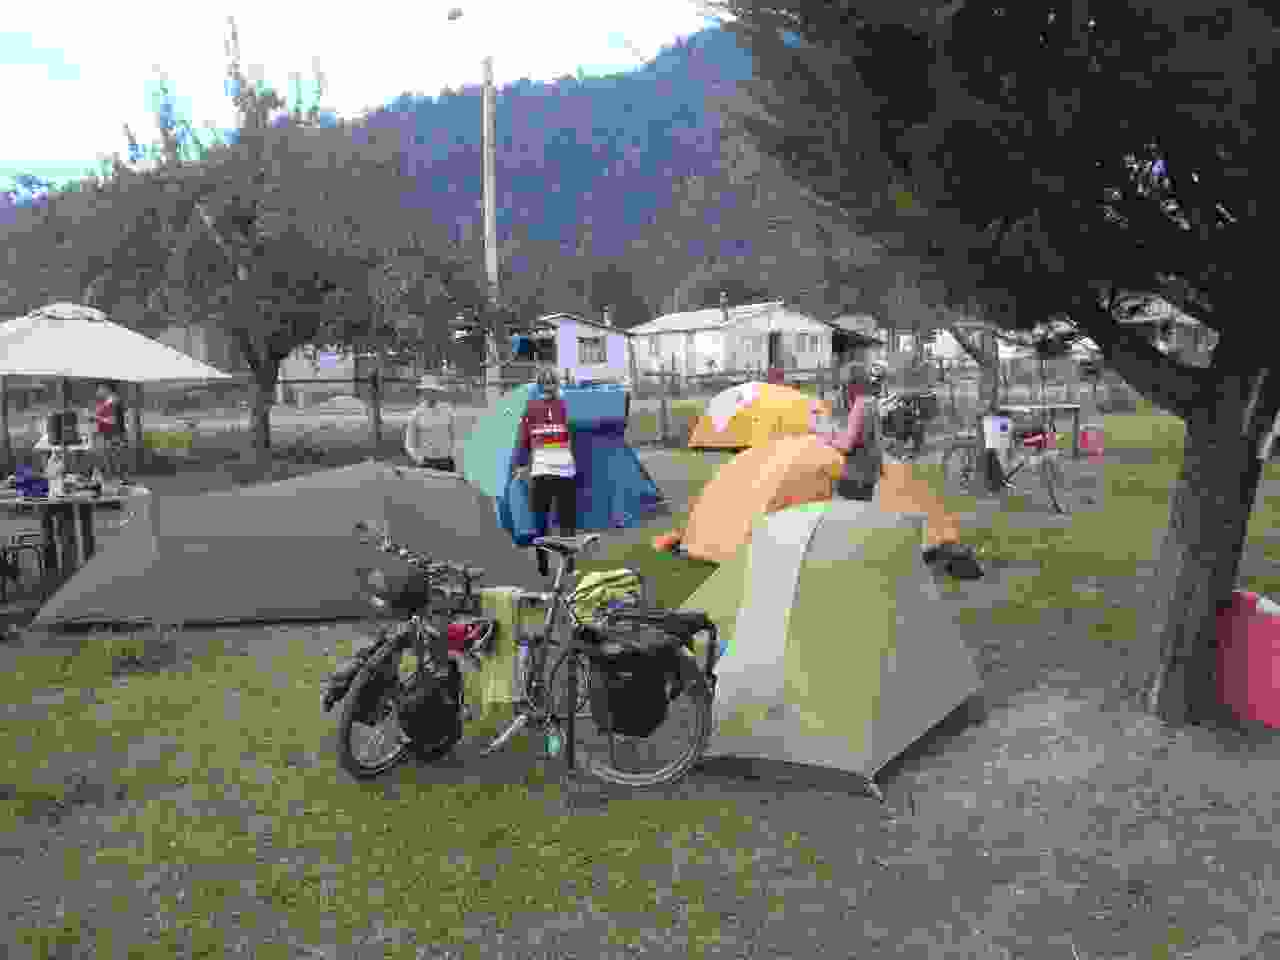
\includegraphics[width=\mywidth]{../wp-content/uploads/2015/02/P2212275.jpg} \end{center}

Deuxième étape jusqu'à Chaiten.
\begin{center} 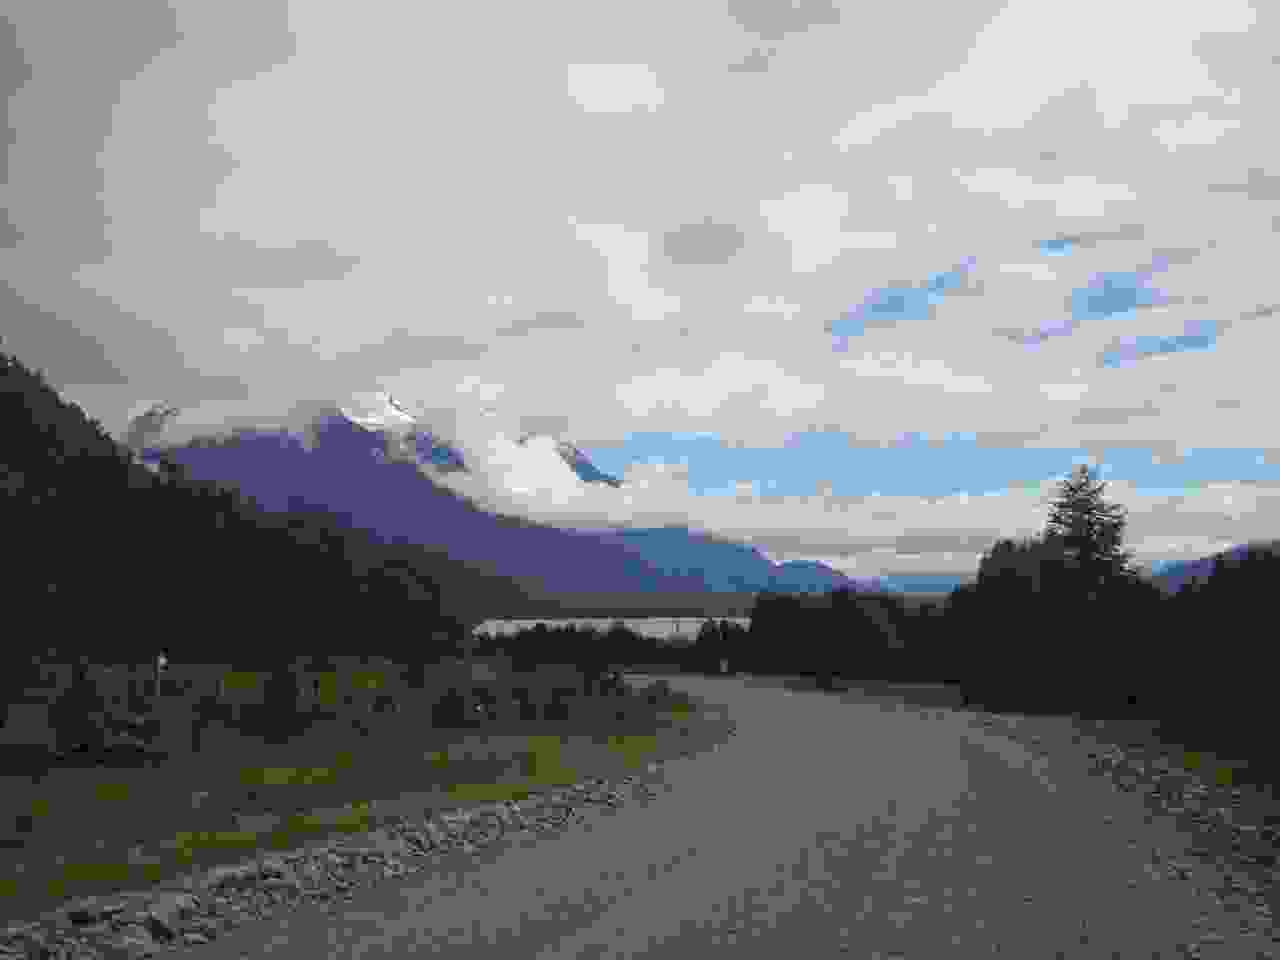
\includegraphics[width=\mywidth]{../wp-content/uploads/2015/02/P2212277.jpg} \end{center}
\begin{center} 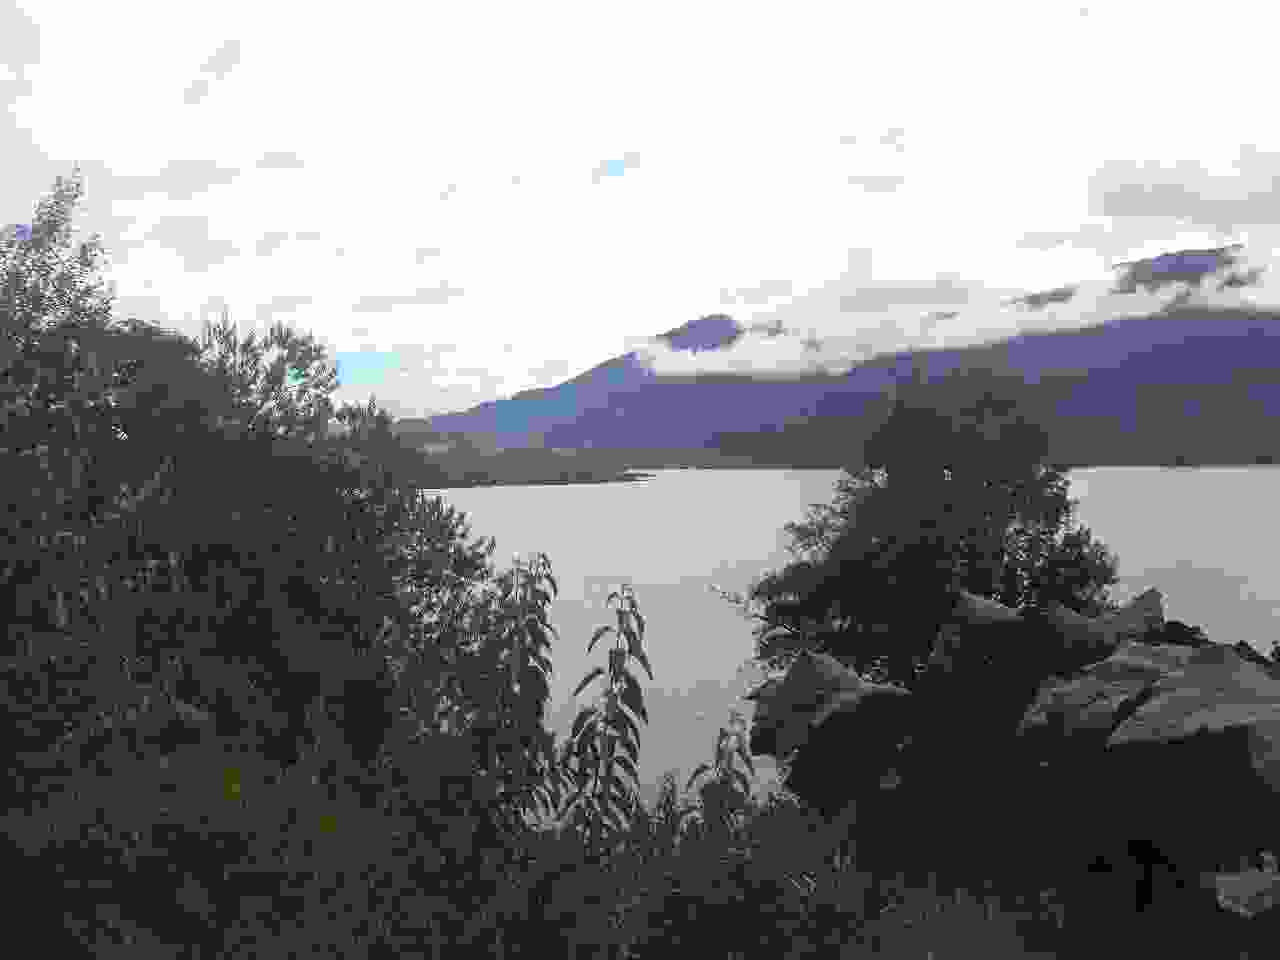
\includegraphics[width=\mywidth]{../wp-content/uploads/2015/02/P2212280.jpg} \end{center}
\begin{center} 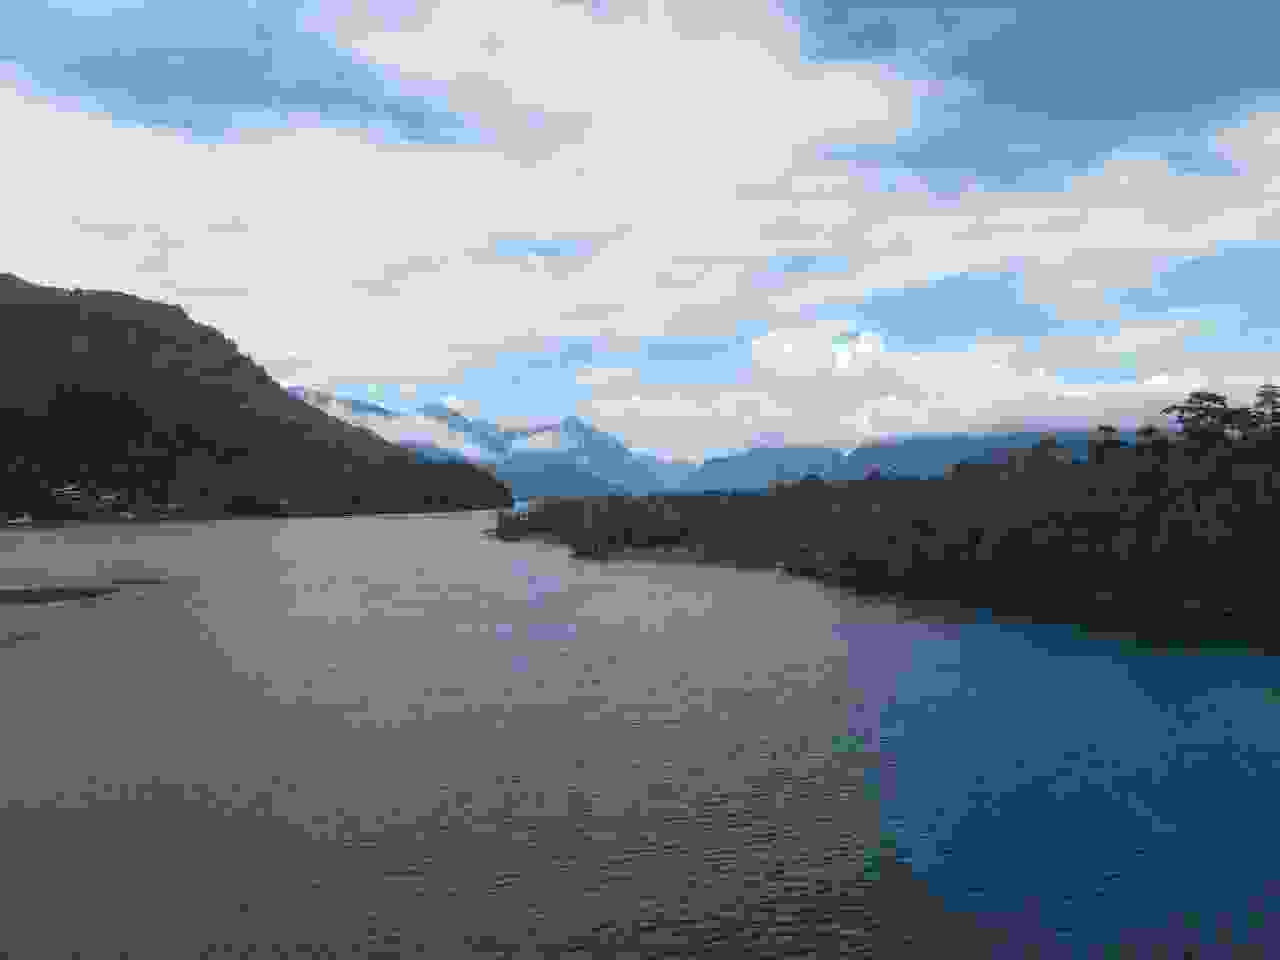
\includegraphics[width=\mywidth]{../wp-content/uploads/2015/02/P2212281.jpg} \end{center}
\begin{center} 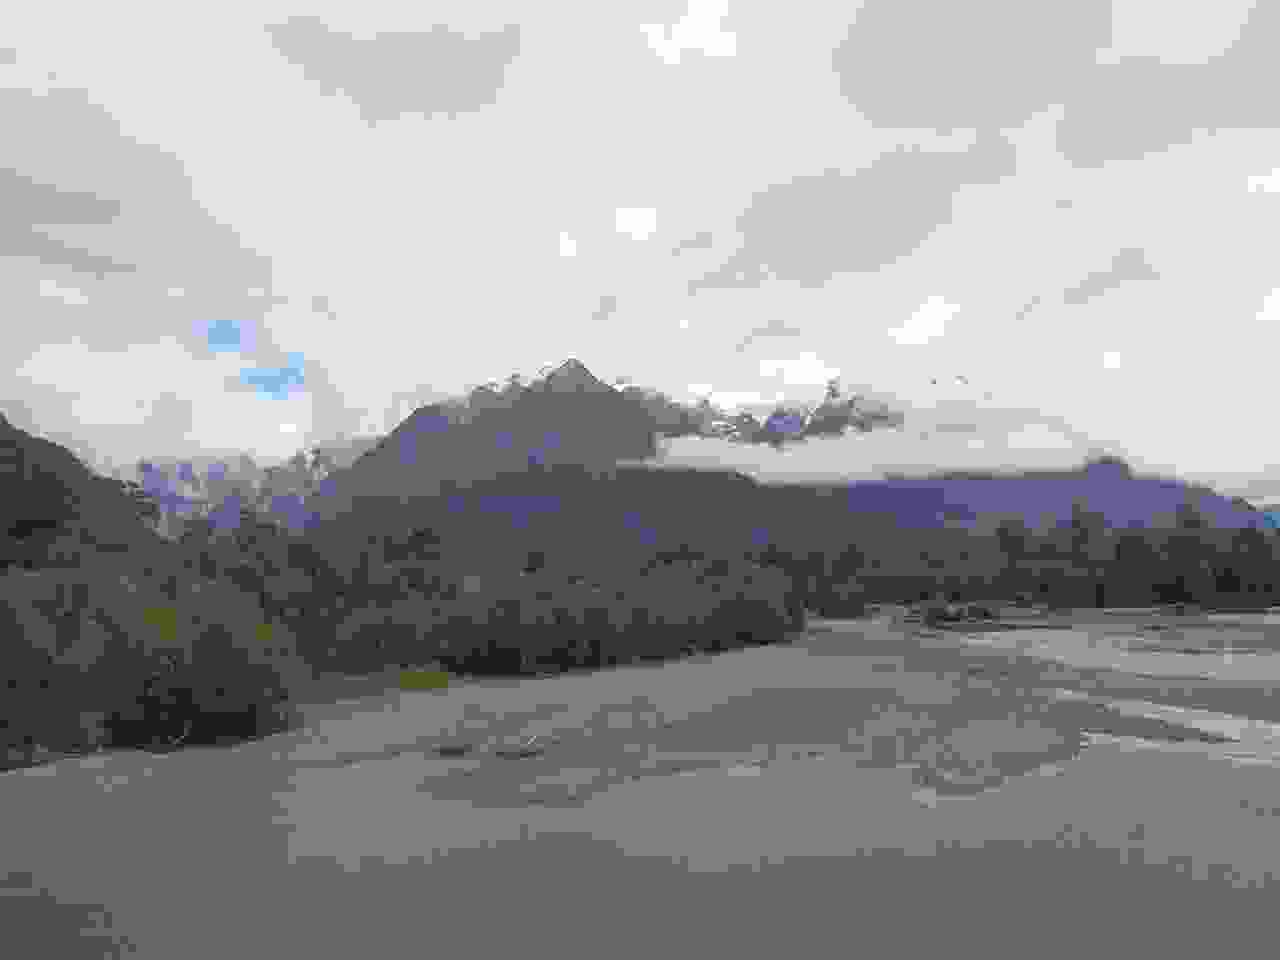
\includegraphics[width=\mywidth]{../wp-content/uploads/2015/02/P2212283.jpg} \end{center}
\begin{center} 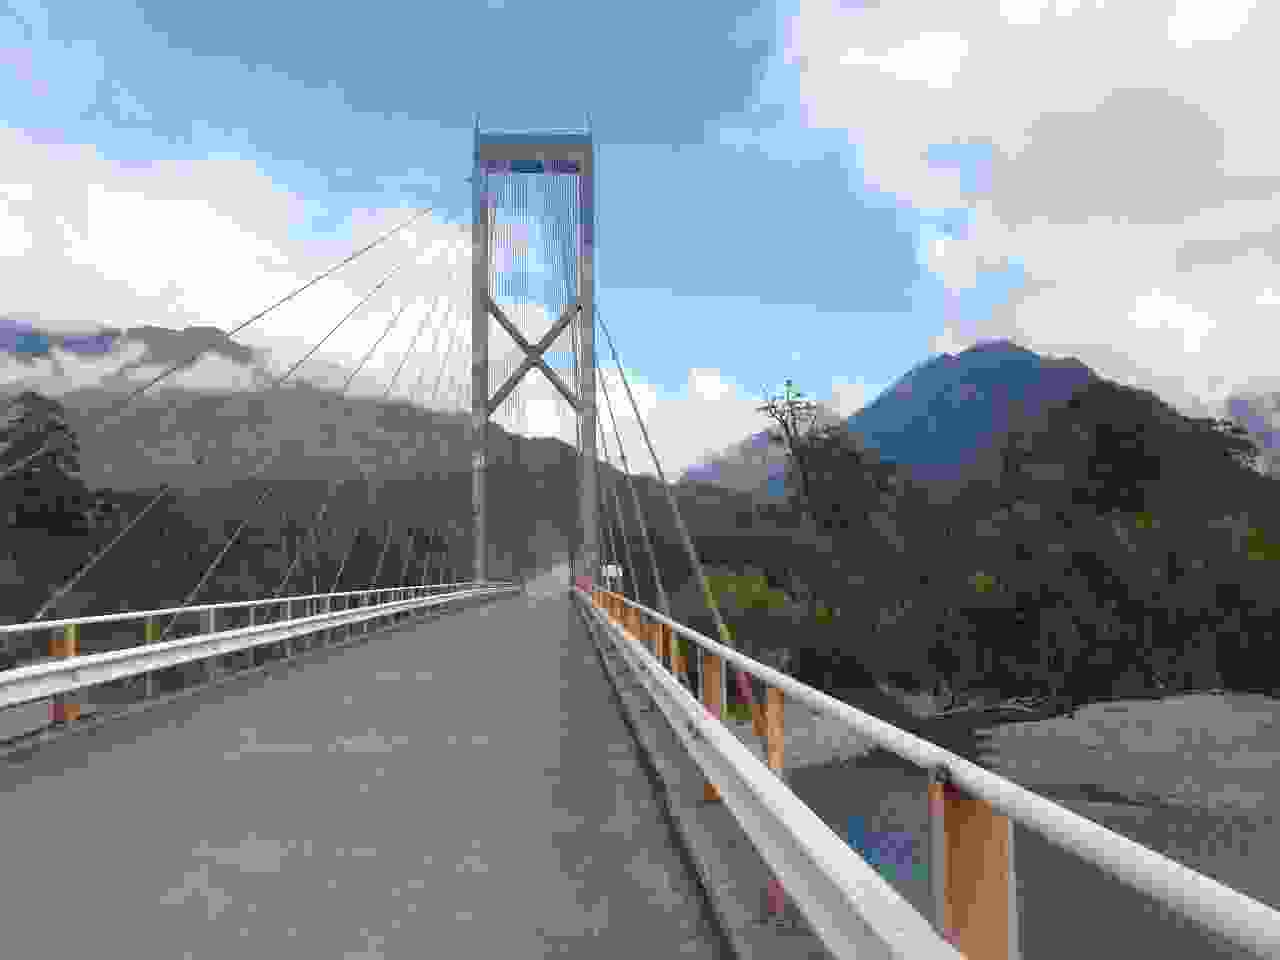
\includegraphics[width=\mywidth]{../wp-content/uploads/2015/02/P2212284.jpg} \end{center}
\begin{center} 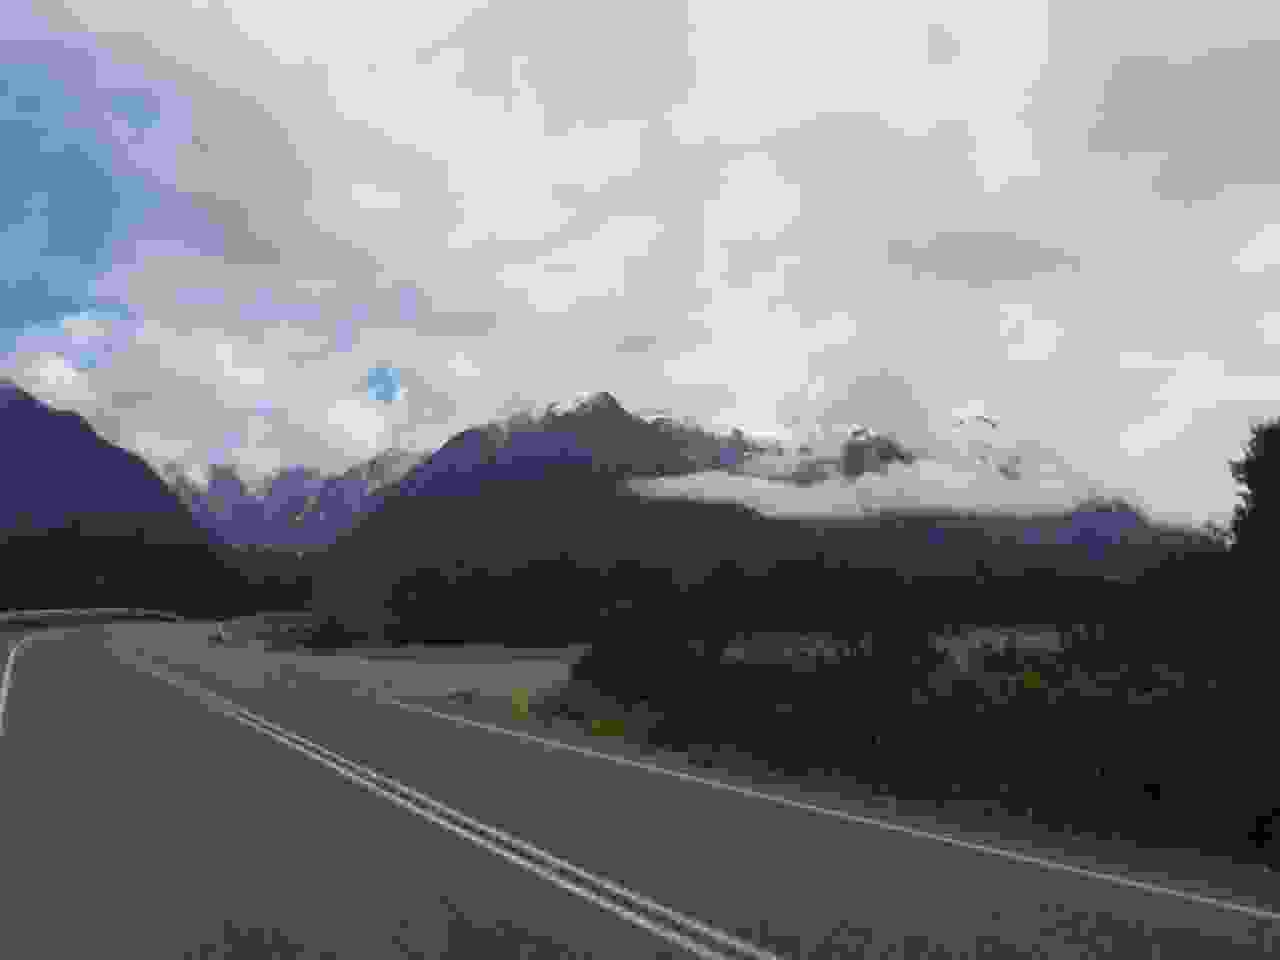
\includegraphics[width=\mywidth]{../wp-content/uploads/2015/02/P2212285.jpg} \end{center}
\begin{center} 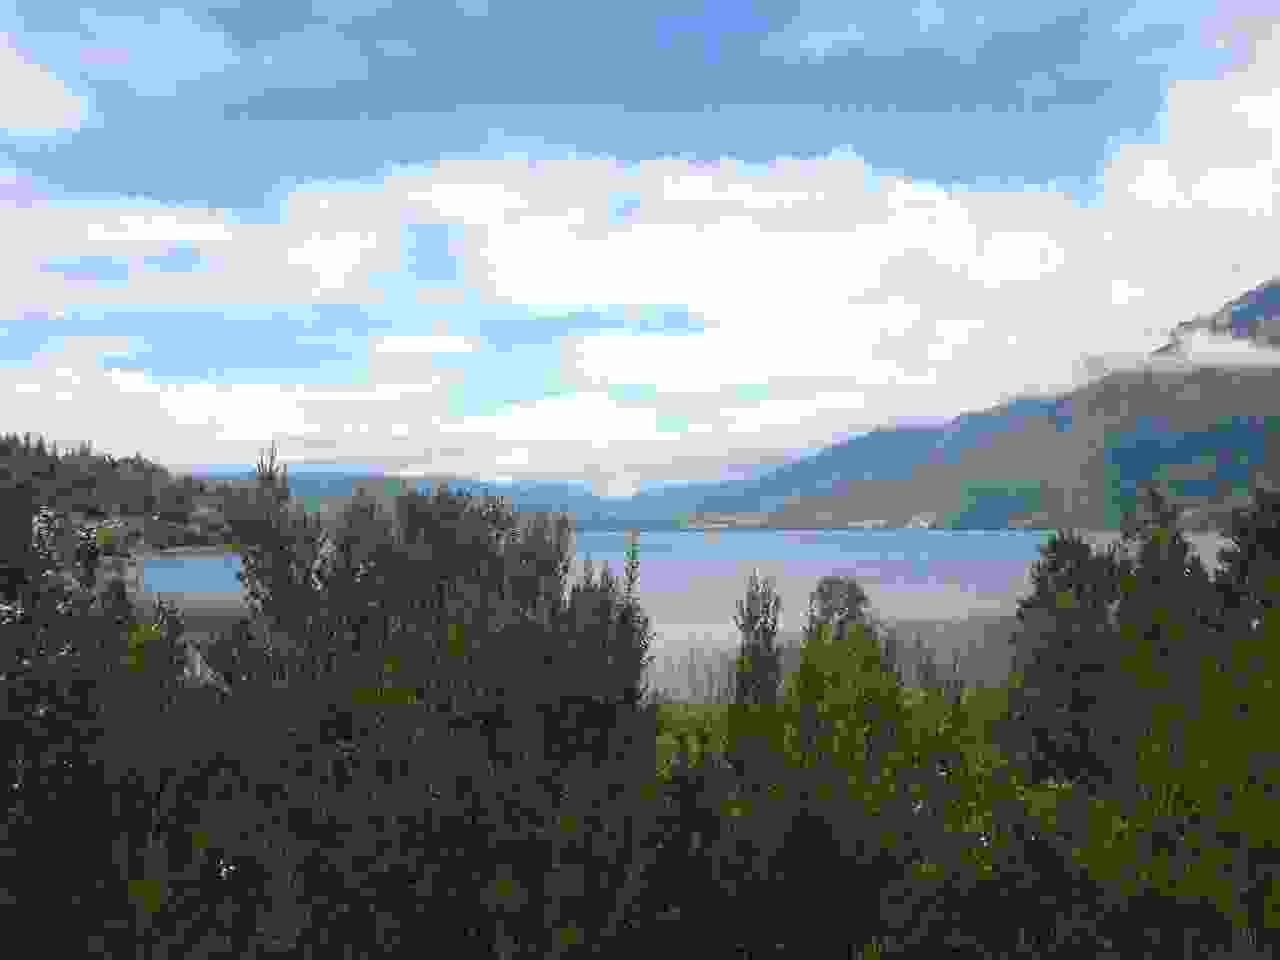
\includegraphics[width=\mywidth]{../wp-content/uploads/2015/02/P2212286.jpg} \end{center}
\begin{center} 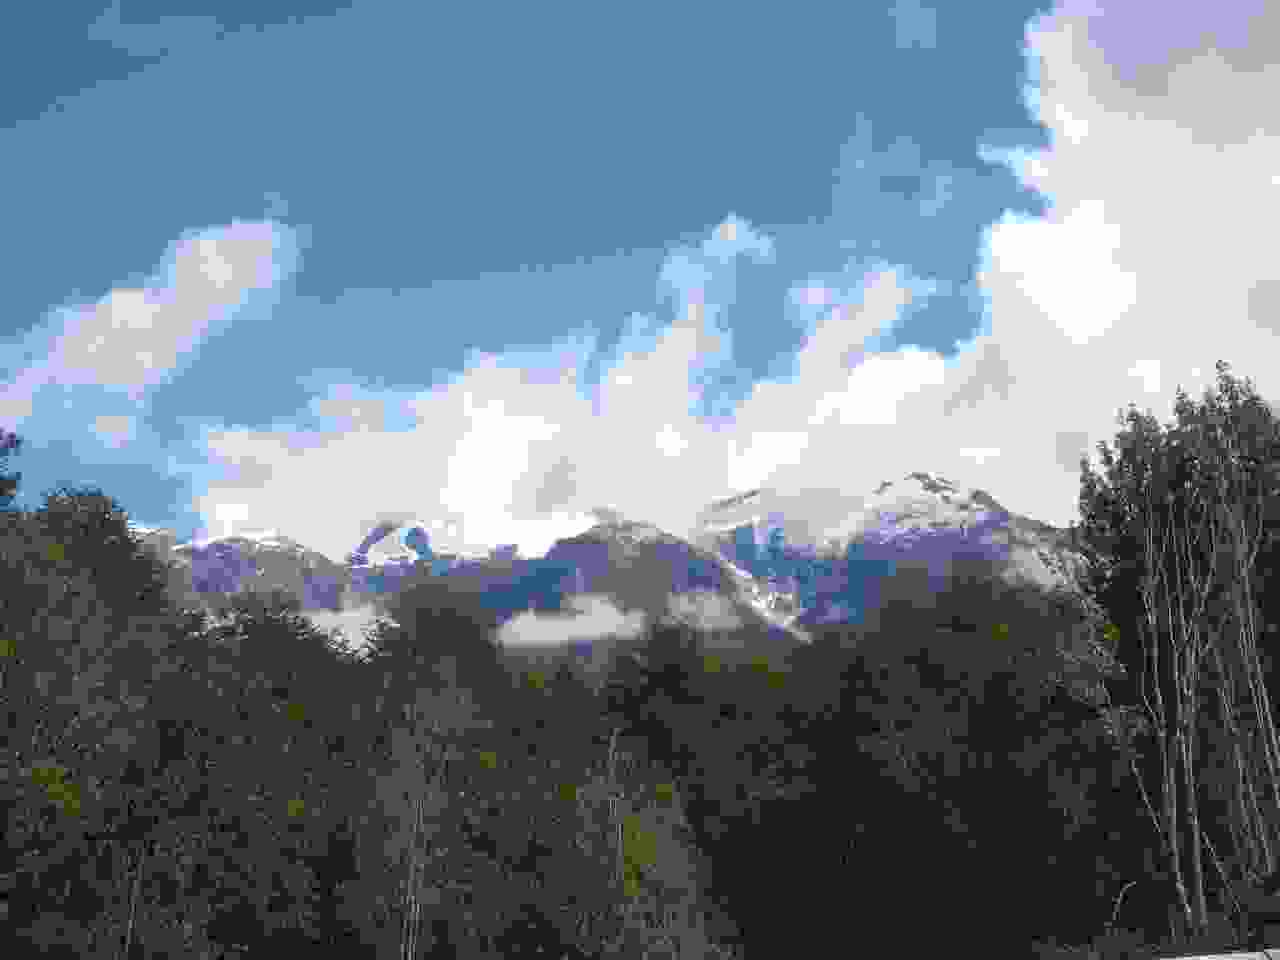
\includegraphics[width=\mywidth]{../wp-content/uploads/2015/02/P2212288.jpg} \end{center}
\vfill
\begin{center} 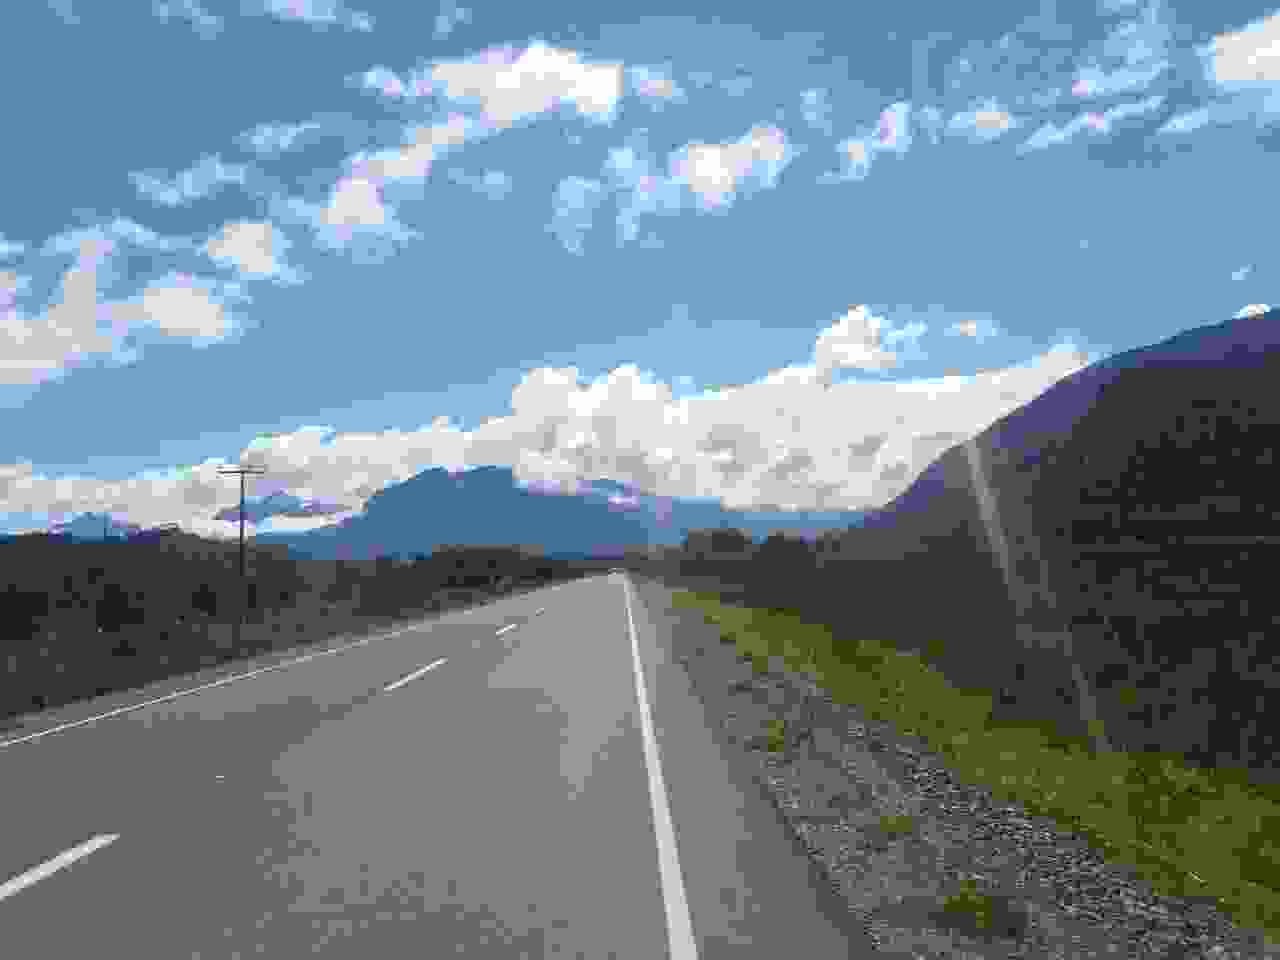
\includegraphics[width=\mywidth]{../wp-content/uploads/2015/02/P2212290.jpg} \end{center}
\vspace{-\topsep}
\vspace{-0.75mm}

\pagebreak
Petit détour pour profiter des thermes d'eau chaude.
\begin{center} 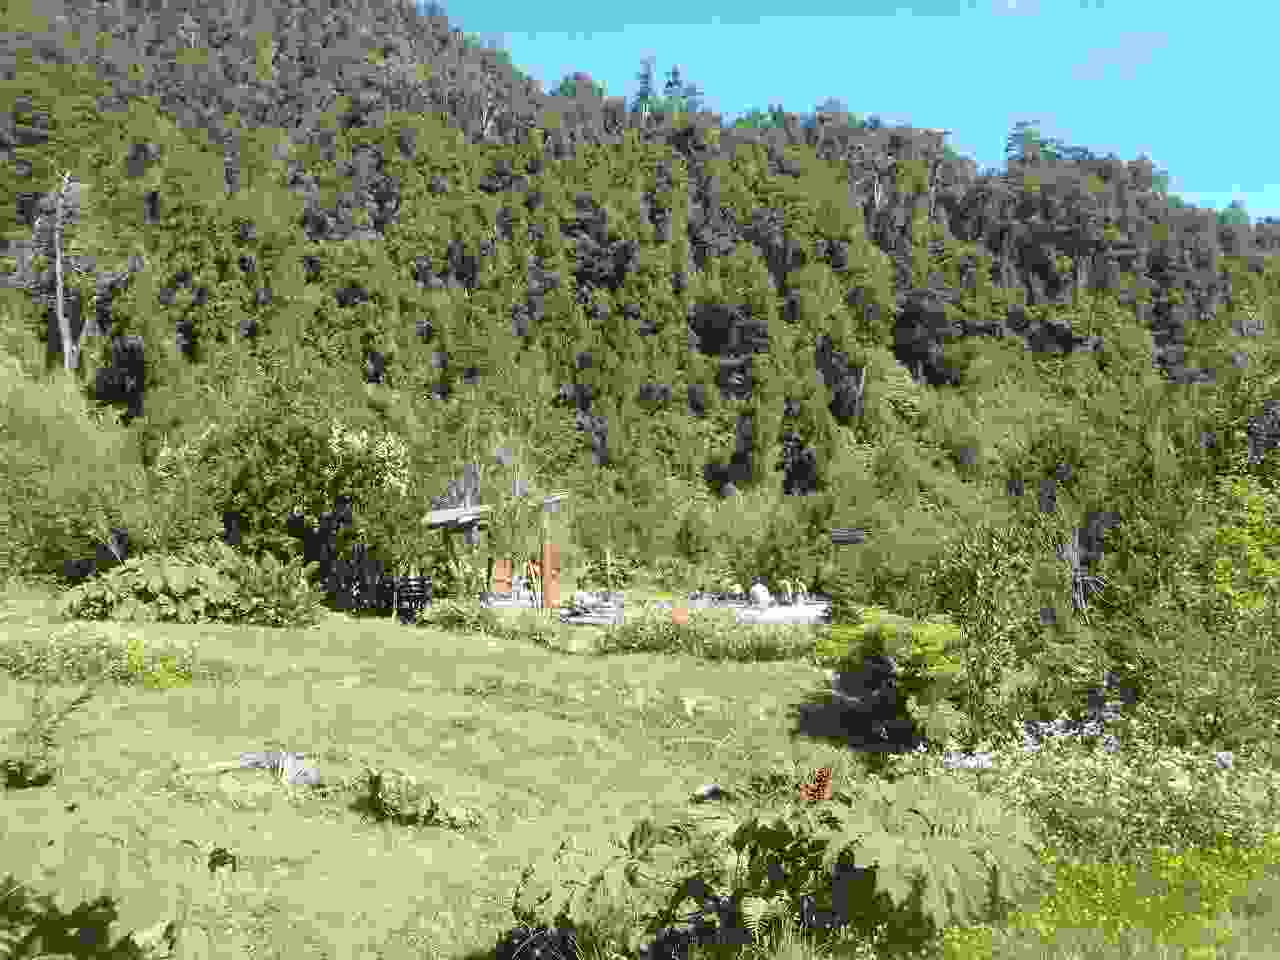
\includegraphics[width=\mywidth]{../wp-content/uploads/2015/02/P2212292.jpg} \end{center}
\begin{center} 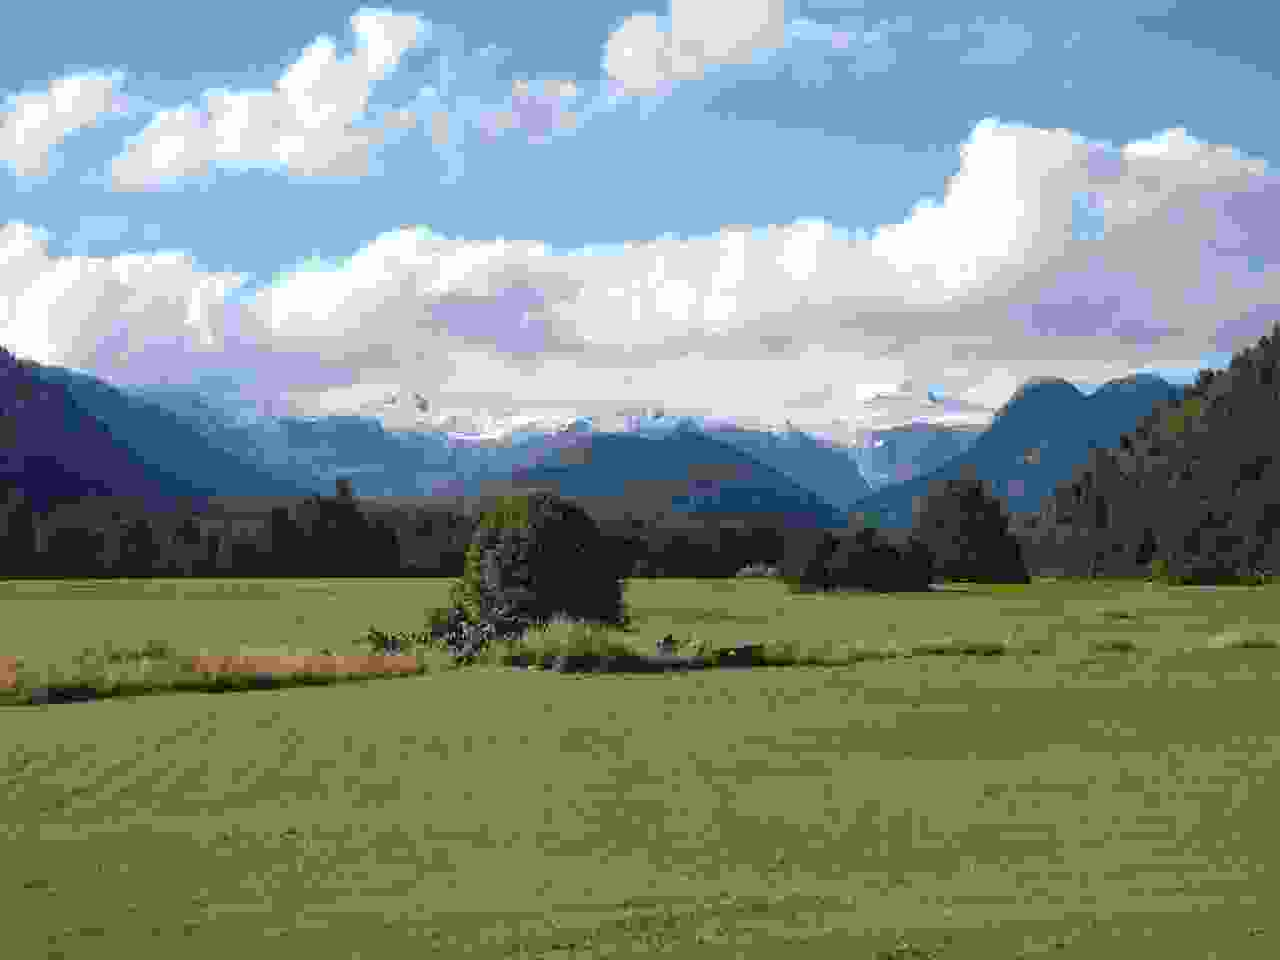
\includegraphics[width=\mywidth]{../wp-content/uploads/2015/02/P2212294.jpg} \end{center}
\begin{center} 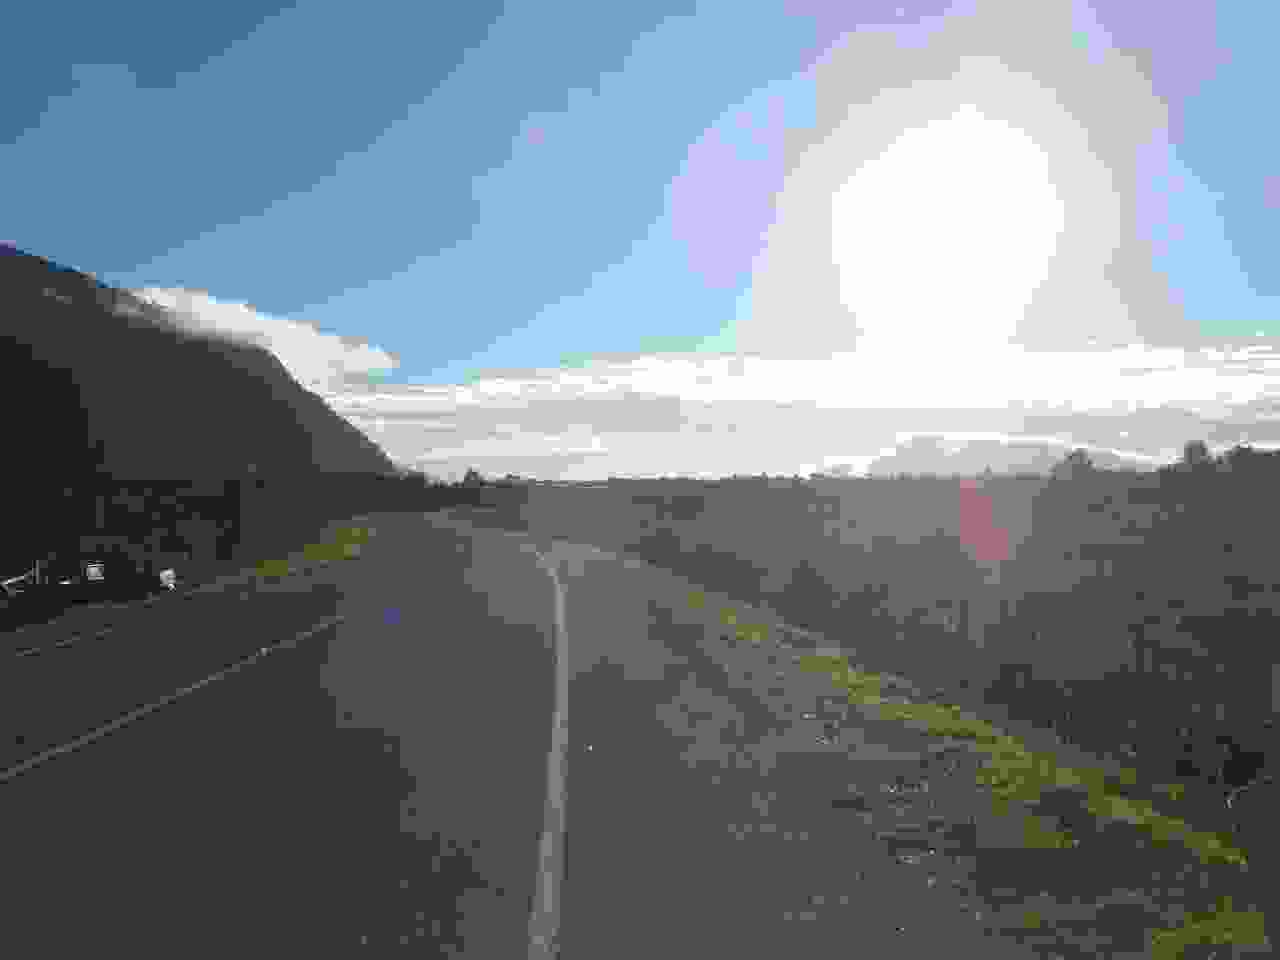
\includegraphics[width=\mywidth]{../wp-content/uploads/2015/02/P2222297.jpg} \end{center}

\`A Chaiten, je suis invité par une famille chilienne rencontrée à une fête locale sur la route.
\begin{center} 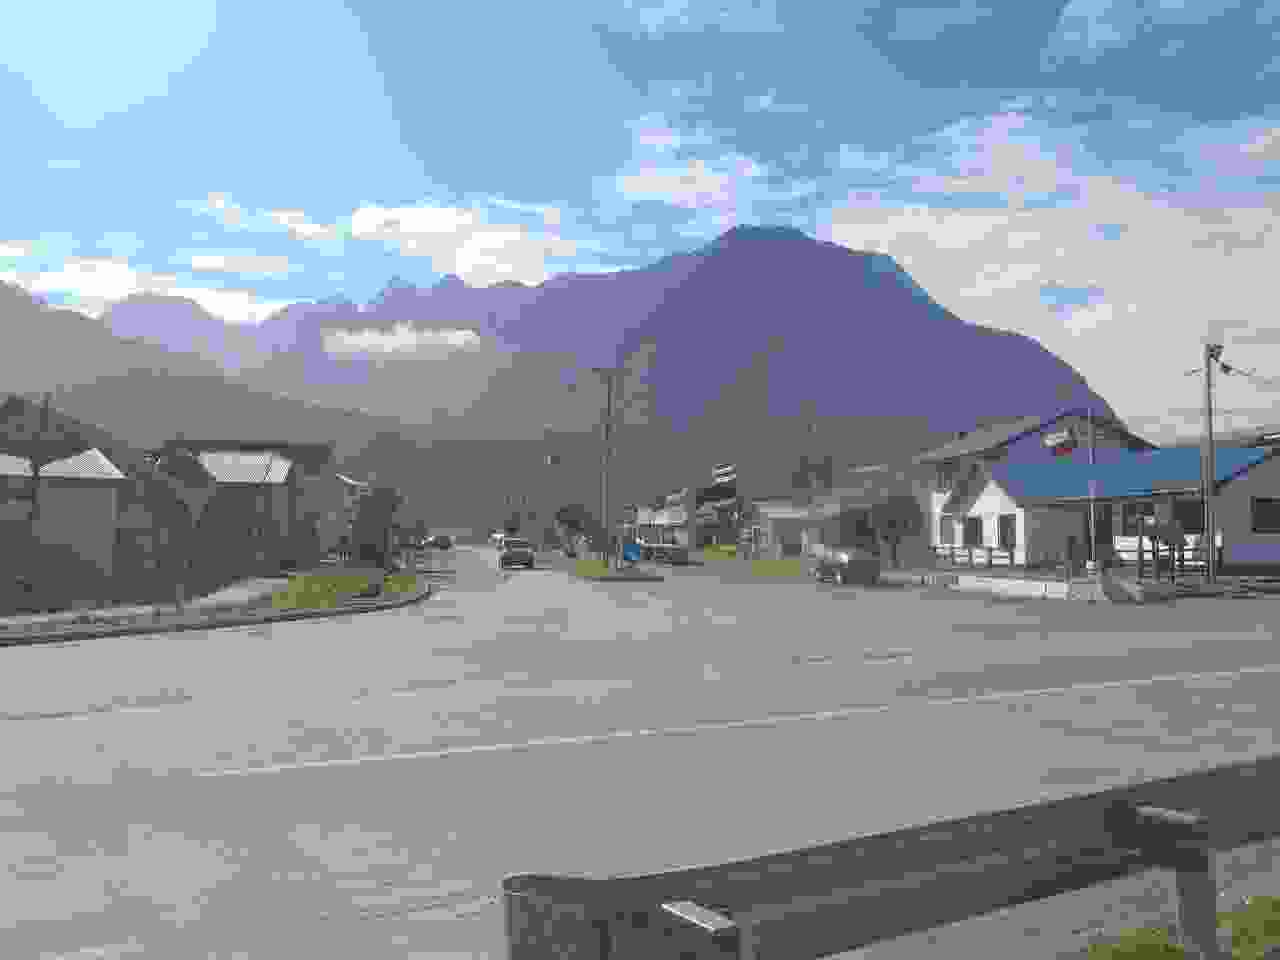
\includegraphics[width=\mywidth]{../wp-content/uploads/2015/02/P2232319.jpg} \end{center}
\vspace{-\topsep}

\pagebreak
~\\
\begin{center} 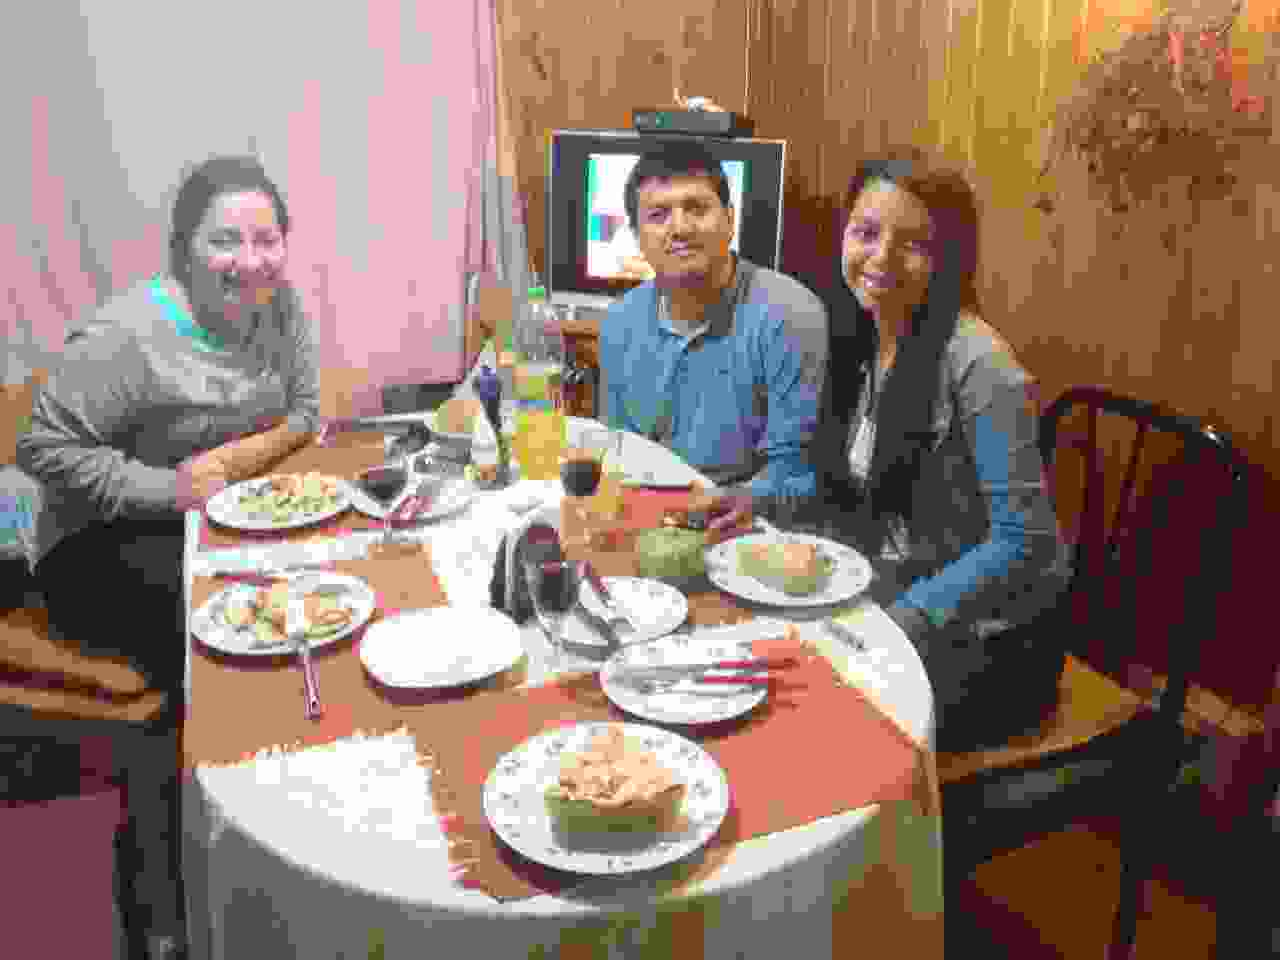
\includegraphics[width=\mywidth]{../wp-content/uploads/2015/02/P2232314.jpg} \end{center}
\begin{center} 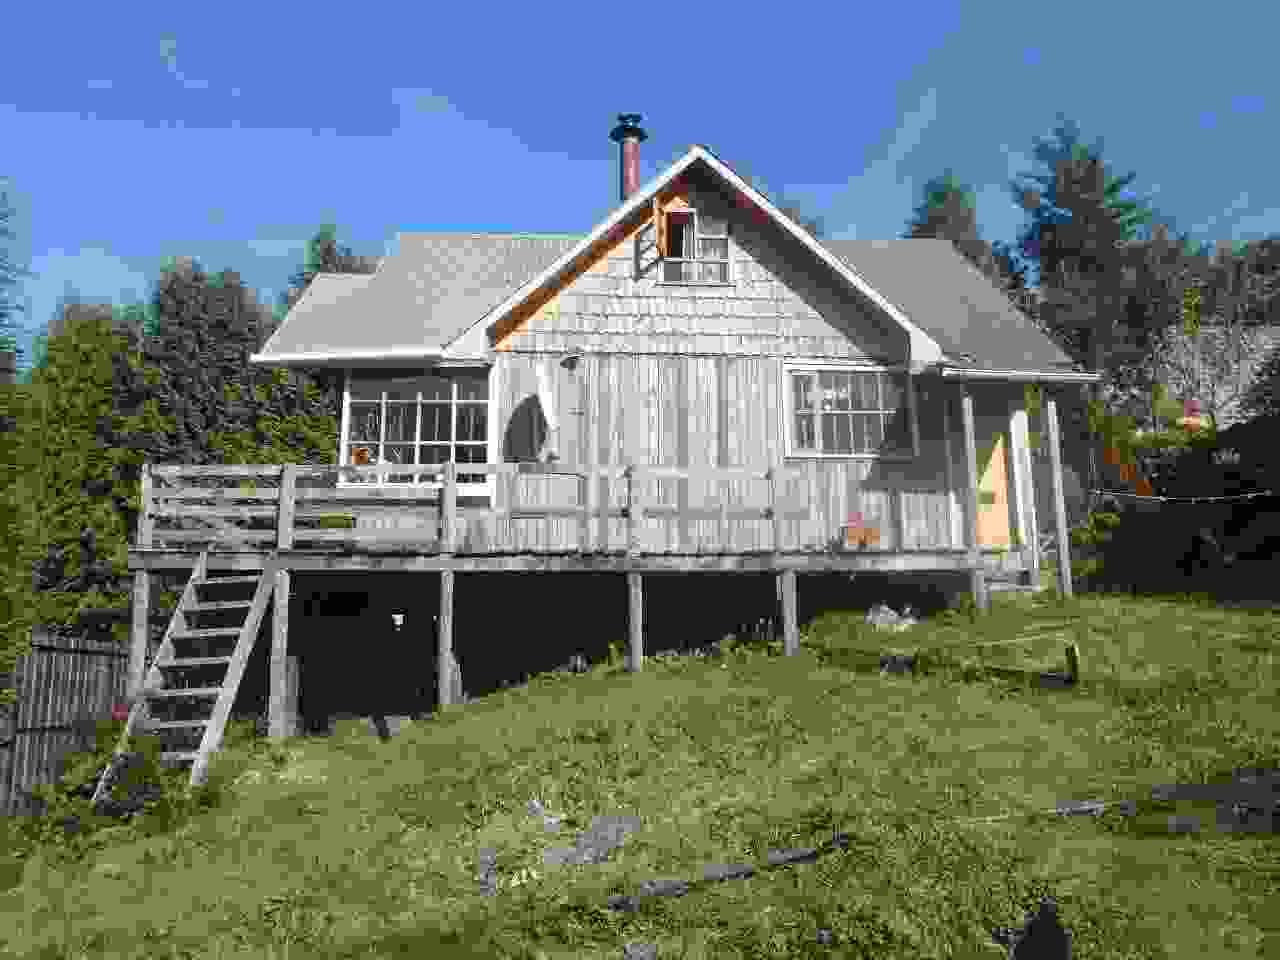
\includegraphics[width=\mywidth]{../wp-content/uploads/2015/02/P2232317.jpg} \end{center}
\vspace{-\topsep}
\vspace{-3mm}

\pagebreak
Du coup, je reste 2 jours ce qui me permet de faire l'ascension du volcan Chaiten, 962m de haut et entré en éruption en 2008.
\begin{center} 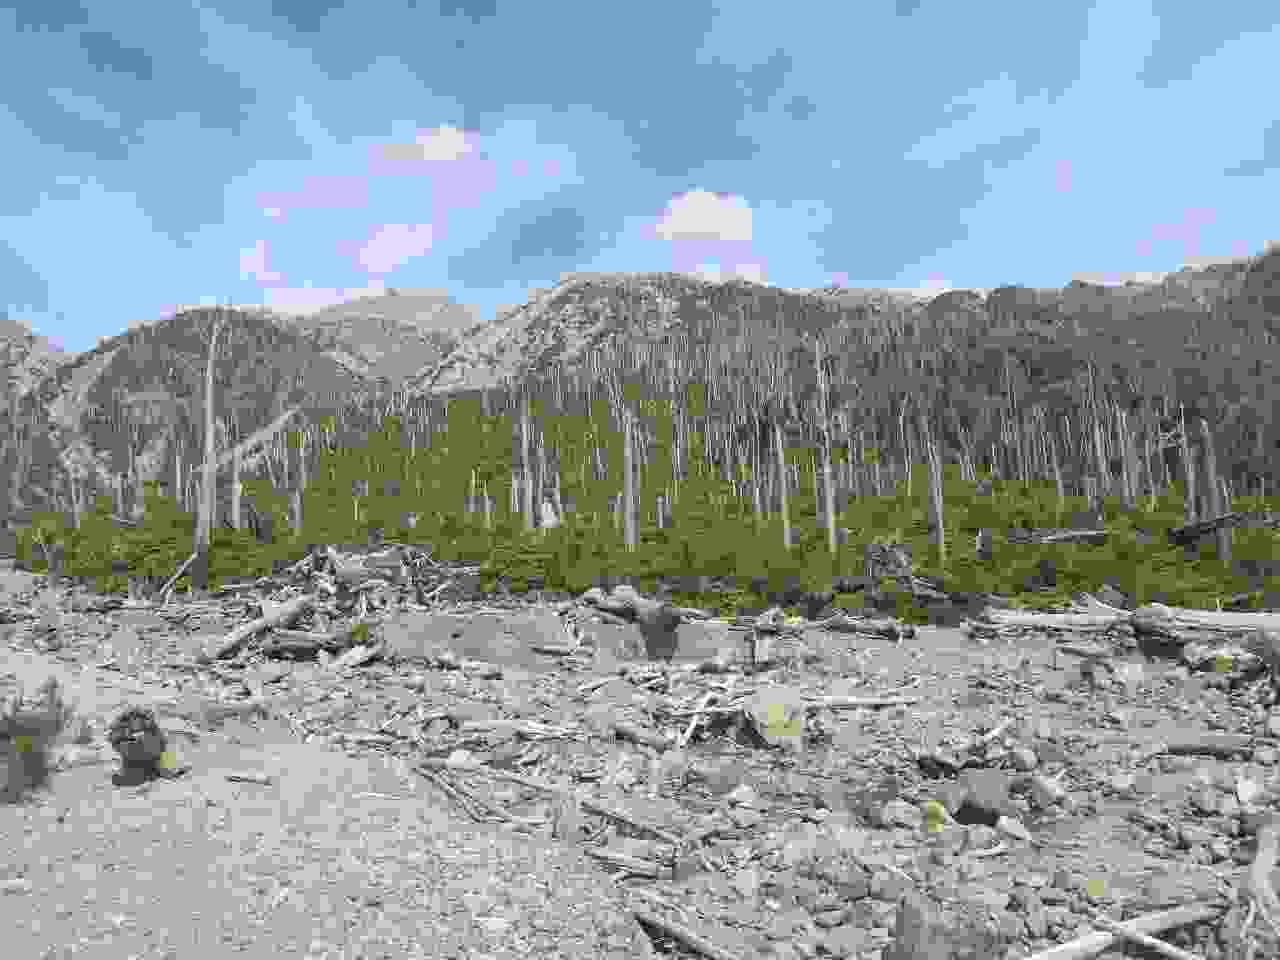
\includegraphics[width=\mywidth]{../wp-content/uploads/2015/02/P2222302.jpg} \end{center}
\begin{center} 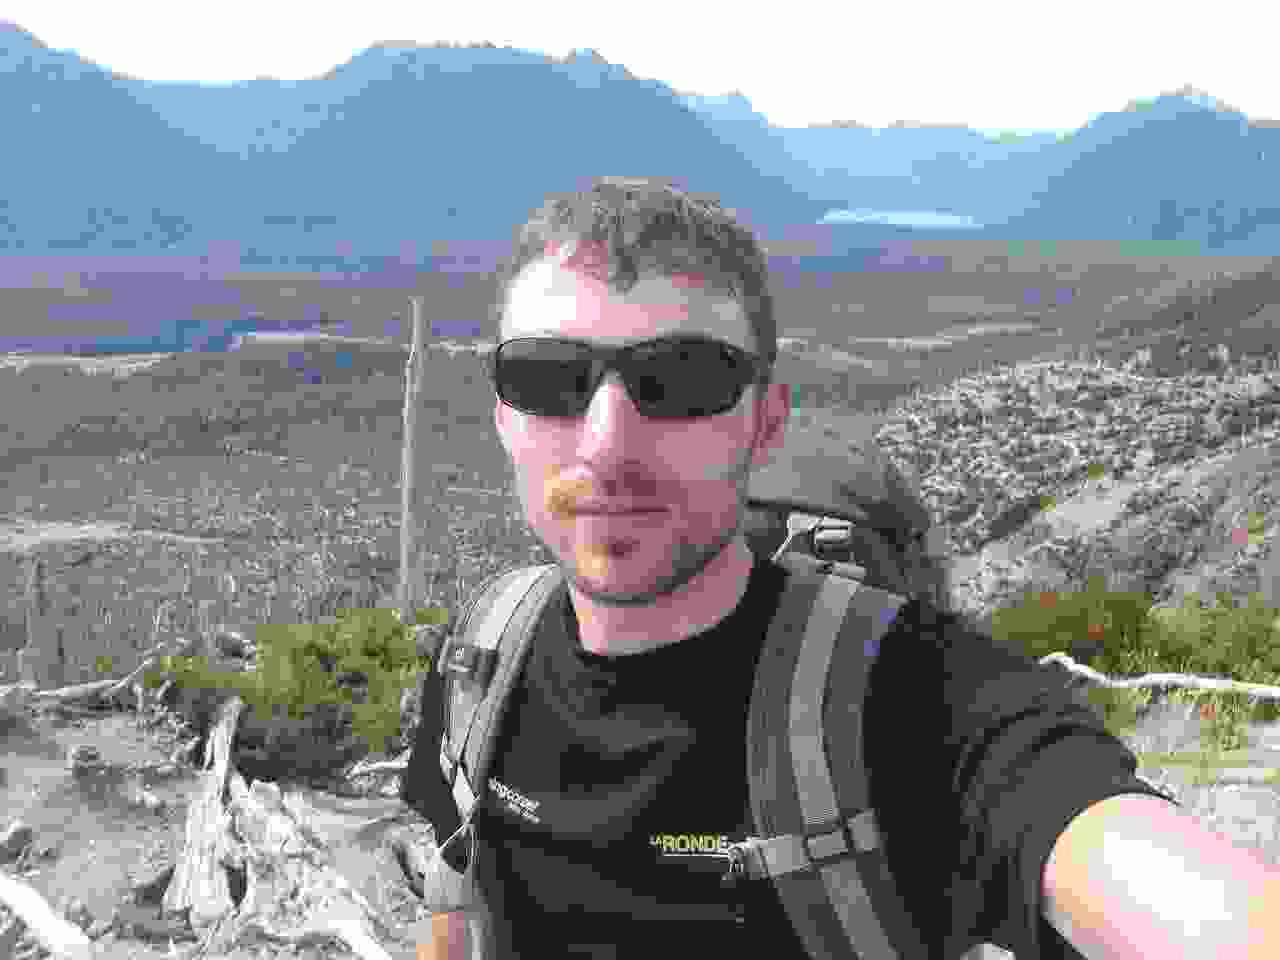
\includegraphics[width=\mywidth]{../wp-content/uploads/2015/02/P2222305.jpg} \end{center}
\begin{center} 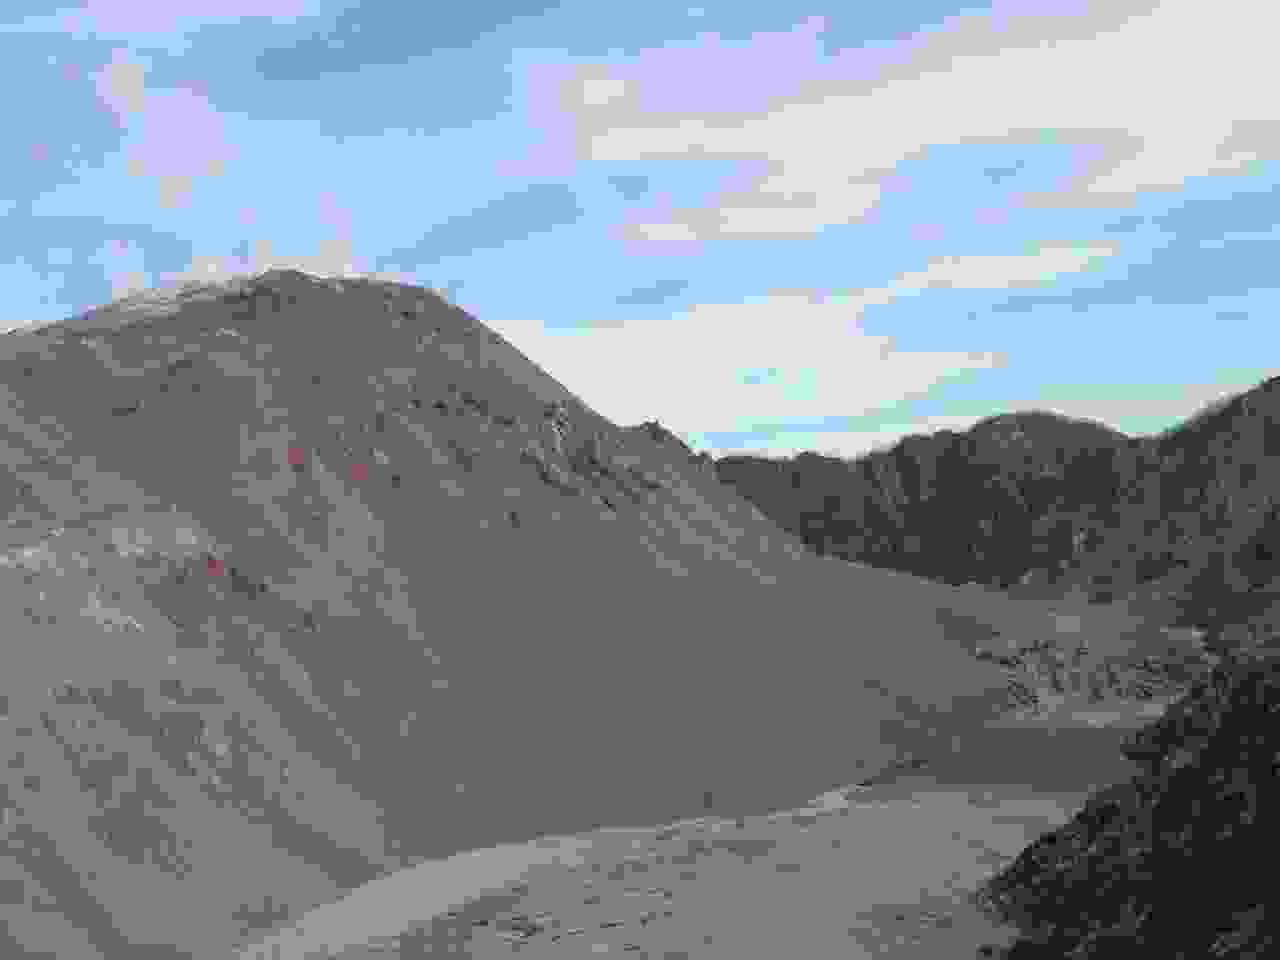
\includegraphics[width=\mywidth]{../wp-content/uploads/2015/02/P2222310.jpg} \end{center}
\begin{center} 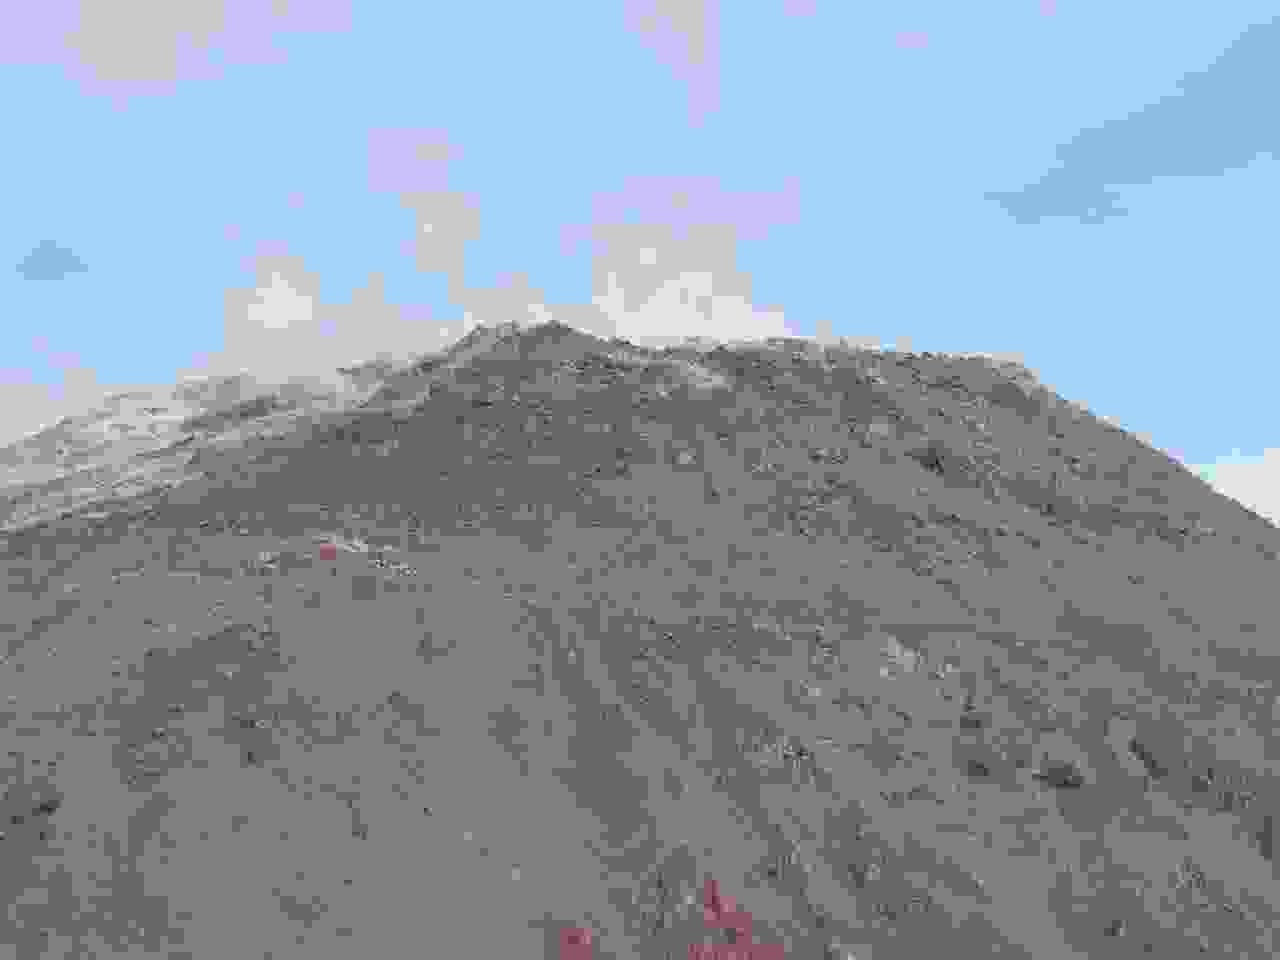
\includegraphics[width=\mywidth]{../wp-content/uploads/2015/02/P2222311.jpg} \end{center}
\begin{center} 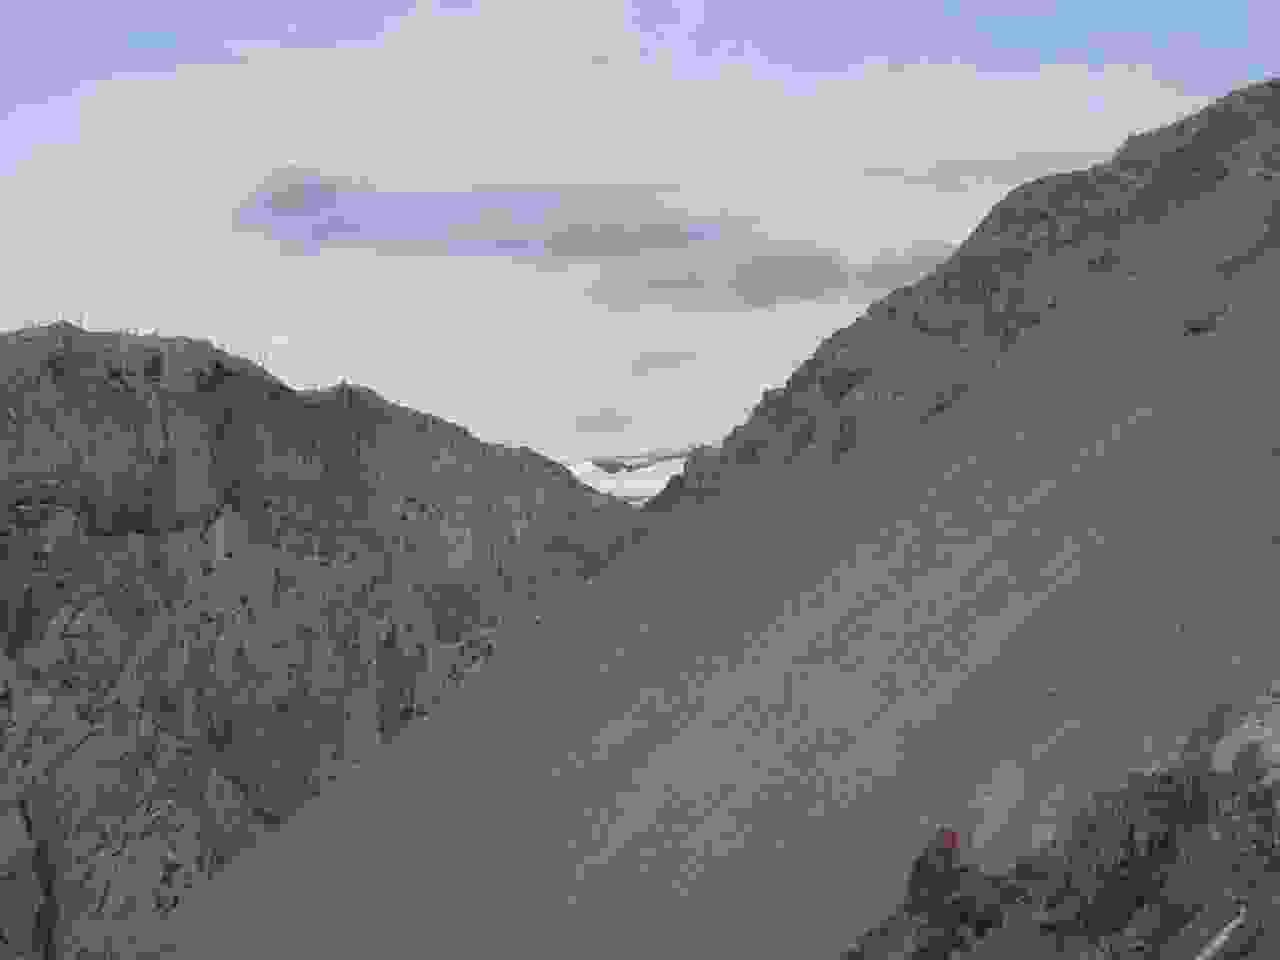
\includegraphics[width=\mywidth]{../wp-content/uploads/2015/02/P2222312.jpg} \end{center}

Je continue direction Caleta Gonzalo, à l'intérieur du parc Pumalin.
\begin{center} 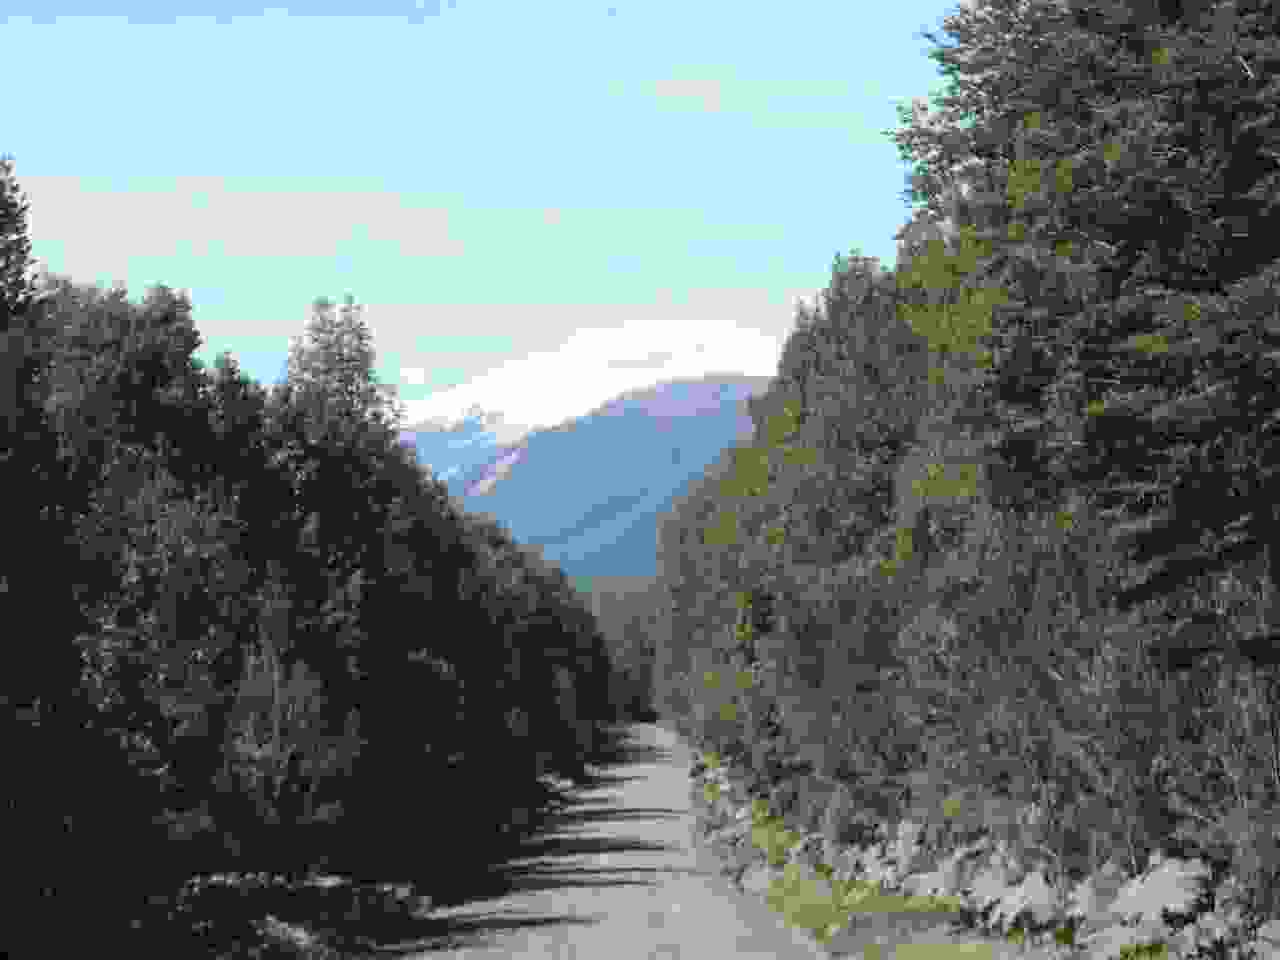
\includegraphics[width=\mywidth]{../wp-content/uploads/2015/02/P2222300.jpg} \end{center}
\begin{center} 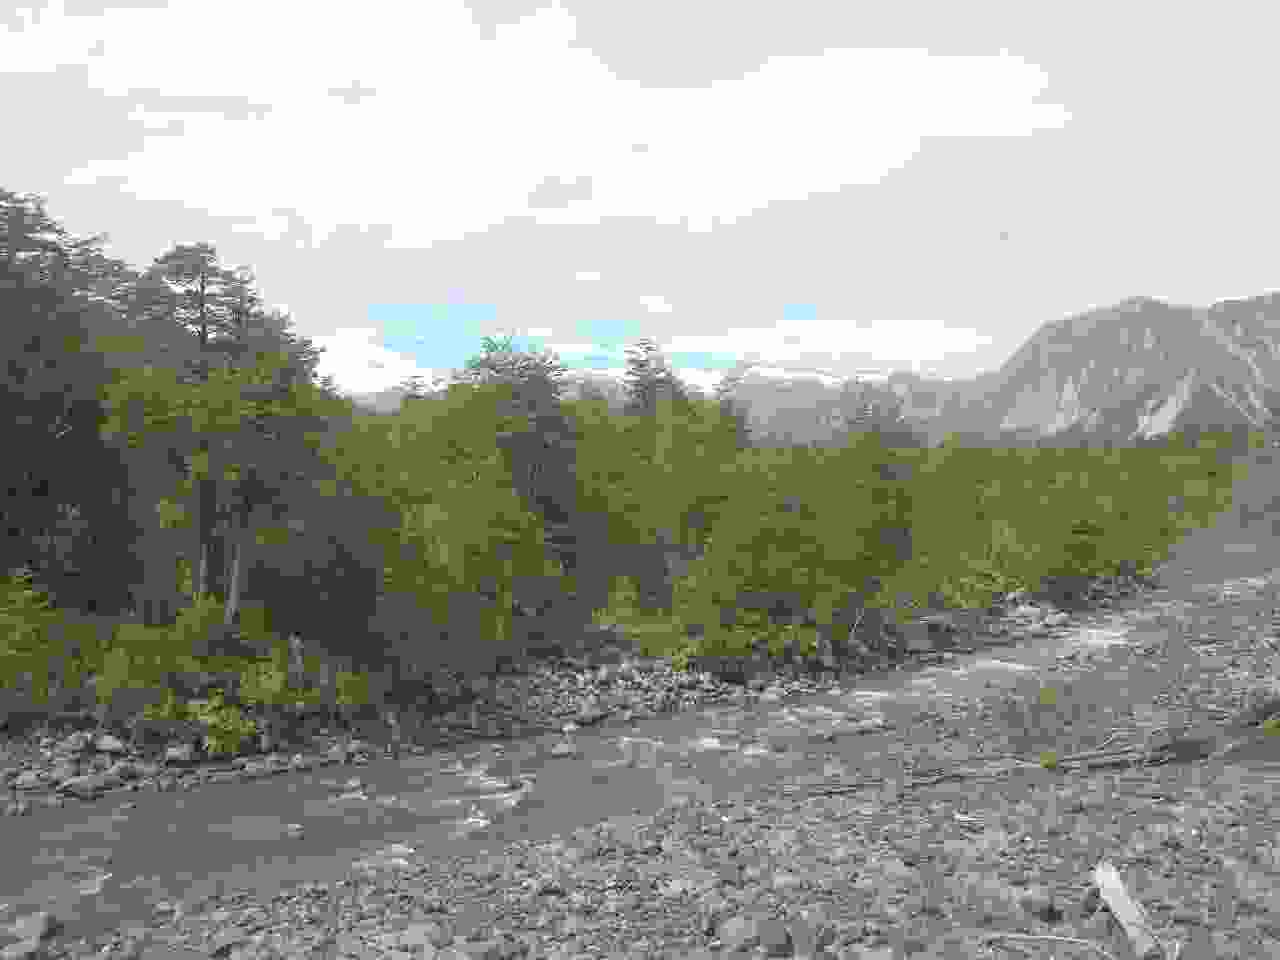
\includegraphics[width=\mywidth]{../wp-content/uploads/2015/02/P2232321.jpg} \end{center}
\begin{center} 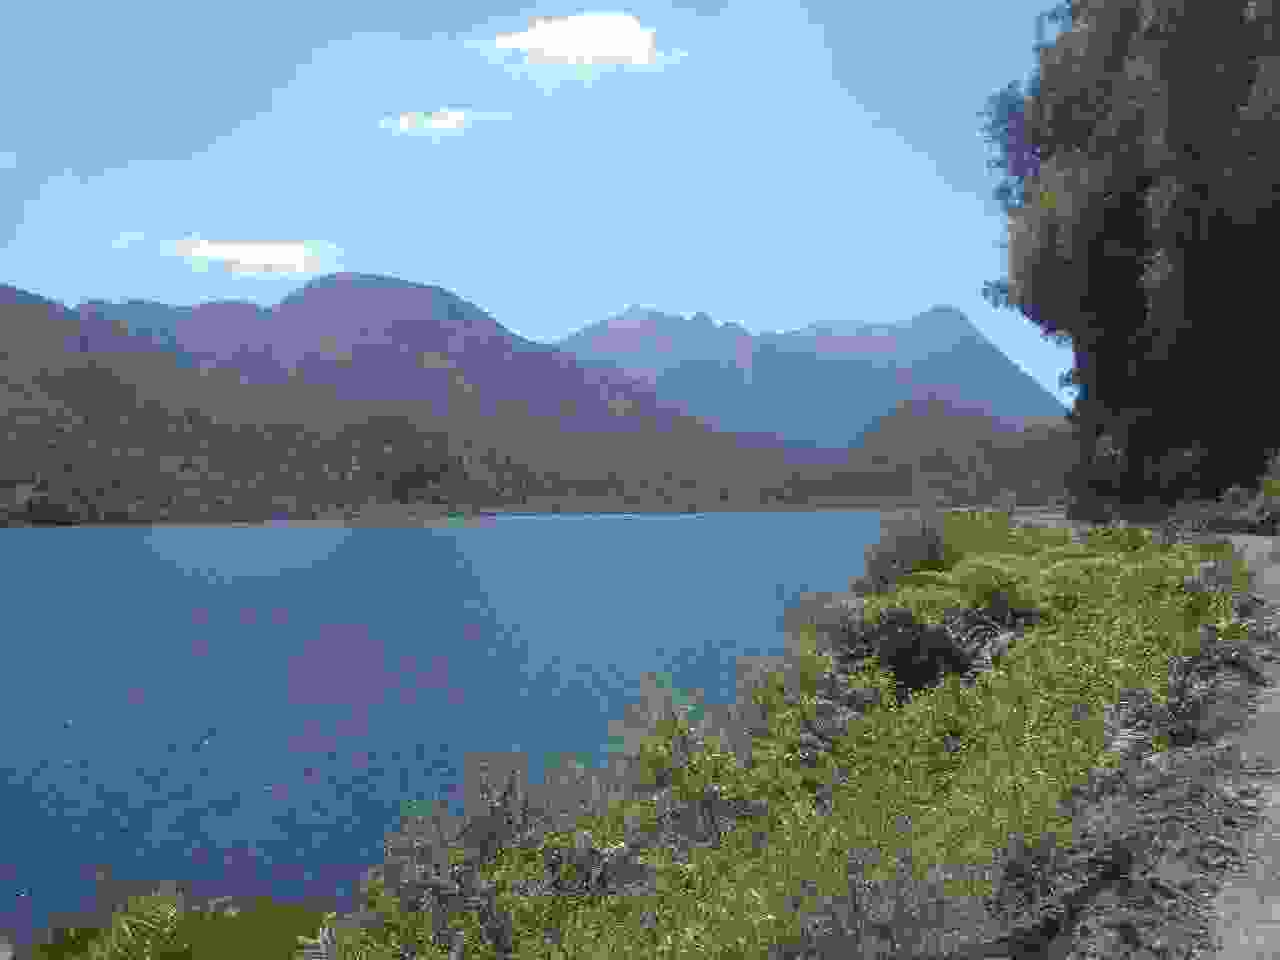
\includegraphics[width=\mywidth]{../wp-content/uploads/2015/02/P2232323.jpg} \end{center}
\begin{center} 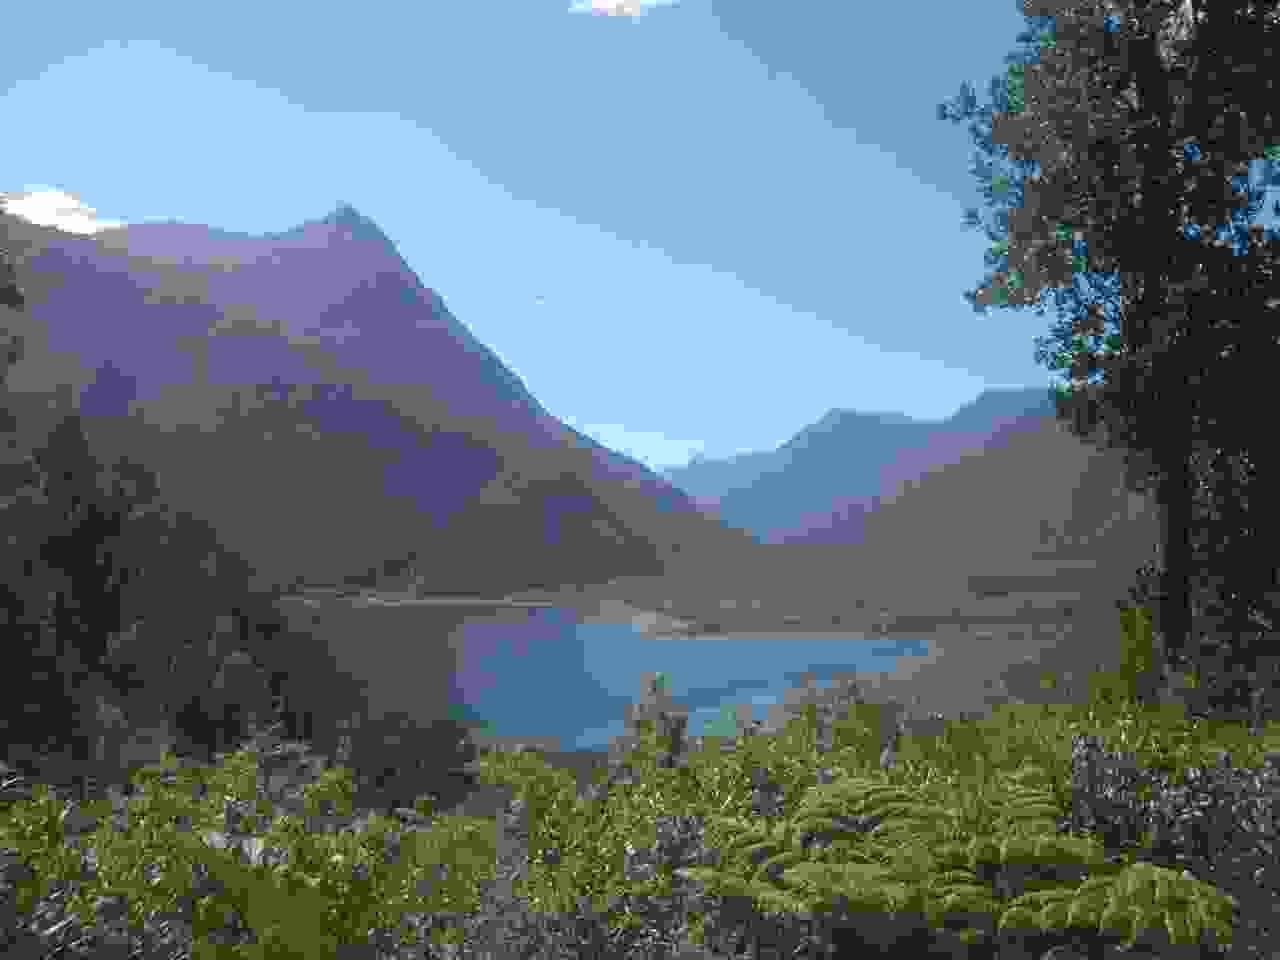
\includegraphics[width=\mywidth]{../wp-content/uploads/2015/02/P2232326.jpg} \end{center}
\vfill
\begin{center} 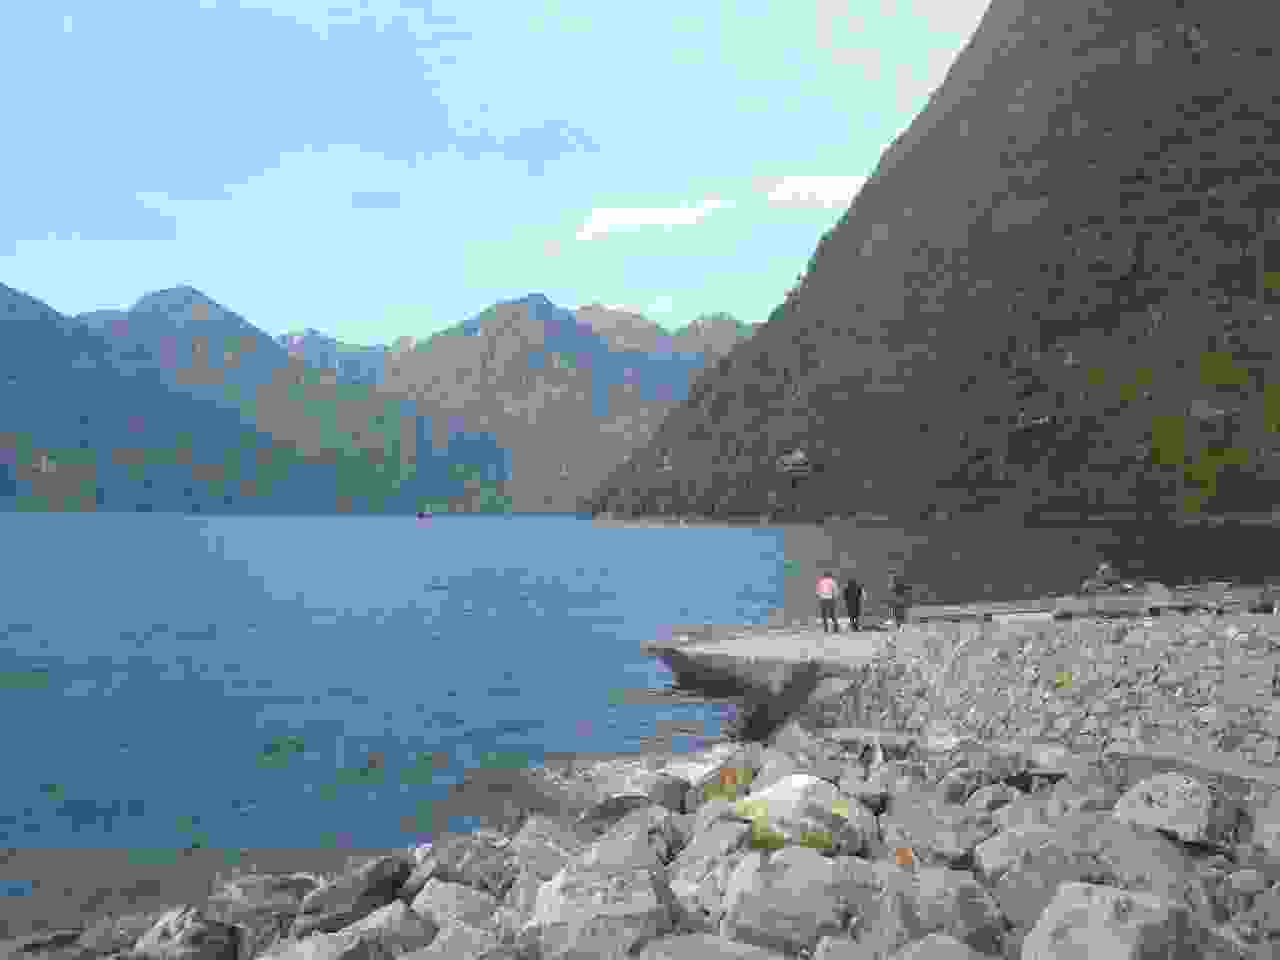
\includegraphics[width=\mywidth]{../wp-content/uploads/2015/02/P2232330.jpg} \end{center}
\vspace{-\topsep}
\vspace{-0.75mm}

\pagebreak
 Journée sur le ferry, encore magnifique entre fjords, montagnes et glaciers.
\begin{center} \includegraphics[width=\mywidth]{../wp-content/uploads/2015/02/P2242333.jpg} \end{center}
\begin{center} \includegraphics[width=\mywidth]{../wp-content/uploads/2015/02/P2242335.jpg} \end{center}
\vspace{-\topsep}
\vspace{-3mm}

\pagebreak
~\\
\begin{center} \includegraphics[width=\mywidth]{../wp-content/uploads/2015/02/P2242338.jpg} \end{center}
\begin{center} \includegraphics[width=\mywidth]{../wp-content/uploads/2015/02/P2242342.jpg} \end{center}
\begin{center} \includegraphics[width=\mywidth]{../wp-content/uploads/2015/02/P2242345.jpg} \end{center}
\begin{center} \includegraphics[width=\mywidth]{../wp-content/uploads/2015/02/P2242347.jpg} \end{center}
\begin{center} \includegraphics[width=\mywidth]{../wp-content/uploads/2015/02/P2242348.jpg} \end{center}
\begin{center} \includegraphics[width=\mywidth]{../wp-content/uploads/2015/02/P2242351.jpg} \end{center}
\begin{center} \includegraphics[width=\mywidth]{../wp-content/uploads/2015/02/P2242354.jpg} \end{center}
\begin{center} \includegraphics[width=\mywidth]{../wp-content/uploads/2015/02/P2242355.jpg} \end{center}
\begin{center} \includegraphics[width=\mywidth]{../wp-content/uploads/2015/02/P2242358.jpg} \end{center}
\begin{center} \includegraphics[width=\mywidth]{../wp-content/uploads/2015/02/P2242359.jpg} \end{center}
\begin{center} \includegraphics[width=\mywidth]{../wp-content/uploads/2015/02/P2242363.jpg} \end{center}
\begin{center} \includegraphics[width=\mywidth]{../wp-content/uploads/2015/02/P2242364.jpg} \end{center}
\begin{center} \includegraphics[width=\mywidth]{../wp-content/uploads/2015/02/P2242366.jpg} \end{center}
\vfill
\begin{center} \includegraphics[width=\mywidth]{../wp-content/uploads/2015/02/P2252370.jpg} \end{center}
\vspace{-\topsep}
\vspace{-0.75mm}

\pagebreak
Sur le bateau, j'ai rencontré un couple de français qui m'a proposé de m'avancer en direction de Puerto Montt. Du coup je suis arrivé plus rapidement en évitant au passage une partie de piste en travaux qui aurait été galère.

 J'en ai profité pour visiter le marché de poissons d'Angelmo.
\begin{center} \includegraphics[width=\mywidth]{../wp-content/uploads/2015/02/P2252373.jpg} \end{center}
\begin{center} \includegraphics[width=\mywidth]{../wp-content/uploads/2015/02/P2252372.jpg} \end{center}
\vspace{-\topsep}
\vspace{-1.25mm}

\pagebreak
  Saumon au beurre dans un des nombreux restaurants du marché.
\begin{center} \includegraphics[width=\mywidth]{../wp-content/uploads/2015/02/P2252376.jpg} \end{center}
\begin{center} \includegraphics[width=\mywidth]{../wp-content/uploads/2015/02/P2252375.jpg} \end{center}
\vspace{-\topsep}
\vspace{-3.25mm}

\pagebreak
  Passage par Puerto Varas au bord du lac Llanquihue, petite ville avec une architecture d'influence allemande.
\begin{center} \includegraphics[width=\mywidth]{../wp-content/uploads/2015/02/P2252379.jpg} \end{center}

Belle route le long du lac avec piste cyclable.
\begin{center} \includegraphics[width=\mywidth]{../wp-content/uploads/2015/02/P2252386.jpg} \end{center}
\begin{center} \includegraphics[width=\mywidth]{../wp-content/uploads/2015/02/P2252387.jpg} \end{center}

 Vues sur le volcan Osorno.
\begin{center} \includegraphics[width=\mywidth]{../wp-content/uploads/2015/02/P2252385.jpg} \end{center}
\vspace{-\topsep}

\pagebreak
~
\begin{center} \includegraphics[width=\mywidth]{../wp-content/uploads/2015/02/P2262390.jpg} \end{center}
\begin{center} \includegraphics[width=\mywidth]{../wp-content/uploads/2015/02/P2262395.jpg} \end{center}
\vspace{-\topsep}
\vspace{-3.25mm}

\pagebreak
Arrivée le lendemain aux chutes de Petrohué.
\begin{center} \includegraphics[width=\mywidth]{../wp-content/uploads/2015/02/P2262401.jpg} \end{center}
\begin{center} \includegraphics[width=\mywidth]{../wp-content/uploads/2015/02/P2262403.jpg} \end{center}
\vspace{-\topsep}
\vspace{-3.25mm}

\pagebreak
 C'est terminé pour le sud du Chili, prochaine étape Santiago puis l'île de Pâques.
\begin{center} \includegraphics[width=\mywidth]{../wp-content/uploads/2015/02/P2282417.jpg} \end{center}
